\documentclass[1p]{elsarticle_modified}
%\bibliographystyle{elsarticle-num}

%\usepackage[colorlinks]{hyperref}
%\usepackage{abbrmath_seonhwa} %\Abb, \Ascr, \Acal ,\Abf, \Afrak
\usepackage{amsfonts}
\usepackage{amssymb}
\usepackage{amsmath}
\usepackage{amsthm}
\usepackage{scalefnt}
\usepackage{amsbsy}
\usepackage{kotex}
\usepackage{caption}
\usepackage{subfig}
\usepackage{color}
\usepackage{graphicx}
\usepackage{xcolor} %% white, black, red, green, blue, cyan, magenta, yellow
\usepackage{float}
\usepackage{setspace}
\usepackage{hyperref}

\usepackage{tikz}
\usetikzlibrary{arrows}

\usepackage{multirow}
\usepackage{array} % fixed length table
\usepackage{hhline}

%%%%%%%%%%%%%%%%%%%%%
\makeatletter
\renewcommand*\env@matrix[1][\arraystretch]{%
	\edef\arraystretch{#1}%
	\hskip -\arraycolsep
	\let\@ifnextchar\new@ifnextchar
	\array{*\c@MaxMatrixCols c}}
\makeatother %https://tex.stackexchange.com/questions/14071/how-can-i-increase-the-line-spacing-in-a-matrix
%%%%%%%%%%%%%%%

\usepackage[normalem]{ulem}

\newcommand{\msout}[1]{\ifmmode\text{\sout{\ensuremath{#1}}}\else\sout{#1}\fi}
%SOURCE: \msout is \stkout macro in https://tex.stackexchange.com/questions/20609/strikeout-in-math-mode

\newcommand{\cancel}[1]{
	\ifmmode
	{\color{red}\msout{#1}}
	\else
	{\color{red}\sout{#1}}
	\fi
}

\newcommand{\add}[1]{
	{\color{blue}\uwave{#1}}
}

\newcommand{\replace}[2]{
	\ifmmode
	{\color{red}\msout{#1}}{\color{blue}\uwave{#2}}
	\else
	{\color{red}\sout{#1}}{\color{blue}\uwave{#2}}
	\fi
}

\newcommand{\Sol}{\mathcal{S}} %segment
\newcommand{\D}{D} %diagram
\newcommand{\A}{\mathcal{A}} %arc


%%%%%%%%%%%%%%%%%%%%%%%%%%%%%5 test

\def\sl{\operatorname{\textup{SL}}(2,\Cbb)}
\def\psl{\operatorname{\textup{PSL}}(2,\Cbb)}
\def\quan{\mkern 1mu \triangleright \mkern 1mu}

\theoremstyle{definition}
\newtheorem{thm}{Theorem}[section]
\newtheorem{prop}[thm]{Proposition}
\newtheorem{lem}[thm]{Lemma}
\newtheorem{ques}[thm]{Question}
\newtheorem{cor}[thm]{Corollary}
\newtheorem{defn}[thm]{Definition}
\newtheorem{exam}[thm]{Example}
\newtheorem{rmk}[thm]{Remark}
\newtheorem{alg}[thm]{Algorithm}

\newcommand{\I}{\sqrt{-1}}
\begin{document}

%\begin{frontmatter}
%
%\title{Boundary parabolic representations of knots up to 8 crossings}
%
%%% Group authors per affiliation:
%\author{Yunhi Cho} 
%\address{Department of Mathematics, University of Seoul, Seoul, Korea}
%\ead{yhcho@uos.ac.kr}
%
%
%\author{Seonhwa Kim} %\fnref{s_kim}}
%\address{Center for Geometry and Physics, Institute for Basic Science, Pohang, 37673, Korea}
%\ead{ryeona17@ibs.re.kr}
%
%\author{Hyuk Kim}
%\address{Department of Mathematical Sciences, Seoul National University, Seoul 08826, Korea}
%\ead{hyukkim@snu.ac.kr}
%
%\author{Seokbeom Yoon}
%\address{Department of Mathematical Sciences, Seoul National University, Seoul, 08826,  Korea}
%\ead{sbyoon15@snu.ac.kr}
%
%\begin{abstract}
%We find all boundary parabolic representation of knots up to 8 crossings.
%
%\end{abstract}
%\begin{keyword}
%    \MSC[2010] 57M25 
%\end{keyword}
%
%\end{frontmatter}

%\linenumbers
%\tableofcontents
%
\newcommand\colored[1]{\textcolor{white}{\rule[-0.35ex]{0.8em}{1.4ex}}\kern-0.8em\color{red} #1}%
%\newcommand\colored[1]{\textcolor{white}{ #1}\kern-2.17ex	\textcolor{white}{ #1}\kern-1.81ex	\textcolor{white}{ #1}\kern-2.15ex\color{red}#1	}

{\Large $\underline{12a_{1041}~(K12a_{1041})}$}

\setlength{\tabcolsep}{10pt}
\renewcommand{\arraystretch}{1.6}
\vspace{1cm}\begin{tabular}{m{100pt}>{\centering\arraybackslash}m{274pt}}
\multirow{5}{120pt}{
	\centering
	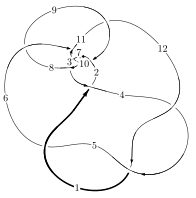
\includegraphics[width=112pt]{../../../GIT/diagram.site/Diagrams/png/1842_12a_1041.png}\\
\ \ \ A knot diagram\footnotemark}&
\allowdisplaybreaks
\textbf{Linearized knot diagam} \\
\cline{2-2}
 &
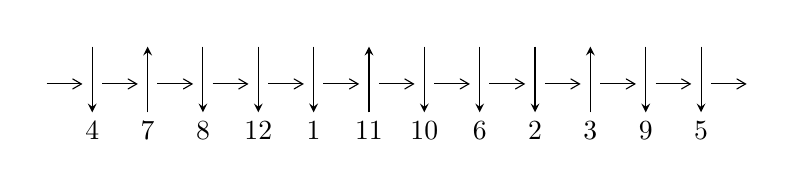
\begin{tikzpicture}[x=20pt, y=17pt]
	% nodes
	\node (C0) at (0, 0) {};
	\node (C1) at (1, 0) {};
	\node (C1U) at (1, +1) {};
	\node (C1D) at (1, -1) {4};

	\node (C2) at (2, 0) {};
	\node (C2U) at (2, +1) {};
	\node (C2D) at (2, -1) {7};

	\node (C3) at (3, 0) {};
	\node (C3U) at (3, +1) {};
	\node (C3D) at (3, -1) {8};

	\node (C4) at (4, 0) {};
	\node (C4U) at (4, +1) {};
	\node (C4D) at (4, -1) {12};

	\node (C5) at (5, 0) {};
	\node (C5U) at (5, +1) {};
	\node (C5D) at (5, -1) {1};

	\node (C6) at (6, 0) {};
	\node (C6U) at (6, +1) {};
	\node (C6D) at (6, -1) {11};

	\node (C7) at (7, 0) {};
	\node (C7U) at (7, +1) {};
	\node (C7D) at (7, -1) {10};

	\node (C8) at (8, 0) {};
	\node (C8U) at (8, +1) {};
	\node (C8D) at (8, -1) {6};

	\node (C9) at (9, 0) {};
	\node (C9U) at (9, +1) {};
	\node (C9D) at (9, -1) {2};

	\node (C10) at (10, 0) {};
	\node (C10U) at (10, +1) {};
	\node (C10D) at (10, -1) {3};

	\node (C11) at (11, 0) {};
	\node (C11U) at (11, +1) {};
	\node (C11D) at (11, -1) {9};

	\node (C12) at (12, 0) {};
	\node (C12U) at (12, +1) {};
	\node (C12D) at (12, -1) {5};
	\node (C13) at (13, 0) {};

	% arrows
	\draw[->,>={angle 60}]
	(C0) edge (C1) (C1) edge (C2) (C2) edge (C3) (C3) edge (C4) (C4) edge (C5) (C5) edge (C6) (C6) edge (C7) (C7) edge (C8) (C8) edge (C9) (C9) edge (C10) (C10) edge (C11) (C11) edge (C12) (C12) edge (C13) ;	\draw[->,>=stealth]
	(C1U) edge (C1D) (C2D) edge (C2U) (C3U) edge (C3D) (C4U) edge (C4D) (C5U) edge (C5D) (C6D) edge (C6U) (C7U) edge (C7D) (C8U) edge (C8D) (C9U) edge (C9D) (C10D) edge (C10U) (C11U) edge (C11D) (C12U) edge (C12D) ;
	\end{tikzpicture} \\
\hhline{~~} \\& 
\textbf{Solving Sequence} \\ \cline{2-2} 
 &
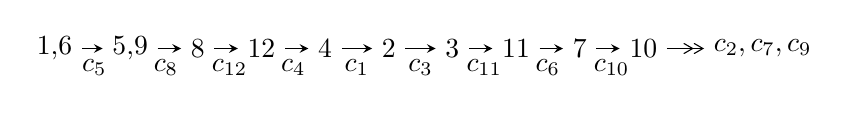
\begin{tikzpicture}[x=23pt, y=7pt]
	% node
	\node (A0) at (-1/8, 0) {1,6};
	\node (A1) at (17/16, 0) {5,9};
	\node (A2) at (17/8, 0) {8};
	\node (A3) at (25/8, 0) {12};
	\node (A4) at (33/8, 0) {4};
	\node (A5) at (41/8, 0) {2};
	\node (A6) at (49/8, 0) {3};
	\node (A7) at (57/8, 0) {11};
	\node (A8) at (65/8, 0) {7};
	\node (A9) at (73/8, 0) {10};
	\node (C1) at (1/2, -1) {$c_{5}$};
	\node (C2) at (13/8, -1) {$c_{8}$};
	\node (C3) at (21/8, -1) {$c_{12}$};
	\node (C4) at (29/8, -1) {$c_{4}$};
	\node (C5) at (37/8, -1) {$c_{1}$};
	\node (C6) at (45/8, -1) {$c_{3}$};
	\node (C7) at (53/8, -1) {$c_{11}$};
	\node (C8) at (61/8, -1) {$c_{6}$};
	\node (C9) at (69/8, -1) {$c_{10}$};
	\node (A10) at (11, 0) {$c_{2},c_{7},c_{9}$};

	% edge
	\draw[->,>=stealth]	
	(A0) edge (A1) (A1) edge (A2) (A2) edge (A3) (A3) edge (A4) (A4) edge (A5) (A5) edge (A6) (A6) edge (A7) (A7) edge (A8) (A8) edge (A9) ;
	\draw[->>,>={angle 60}]	
	(A9) edge (A10);
\end{tikzpicture} \\ 

\end{tabular} \\

\footnotetext{
The image of knot diagram is generated by the software ``\textbf{Draw programme}" developed by Andrew Bartholomew(\url{http://www.layer8.co.uk/maths/draw/index.htm\#Running-draw}), where we modified some parts for our purpose(\url{https://github.com/CATsTAILs/LinksPainter}).
}\phantom \\ \newline 
\centering \textbf{Ideals for irreducible components\footnotemark of $X_{\text{par}}$} 
 
\begin{align*}
I^u_{1}&=\langle 
-1038957476023 u^{54}-8812866915448 u^{53}+\cdots+12177825868 b+10129039394368,\\
\phantom{I^u_{1}}&\phantom{= \langle  }-1082675116975 u^{54}-10377141014923 u^{53}+\cdots+12177825868 a+22705250521701,\\
\phantom{I^u_{1}}&\phantom{= \langle  }u^{55}+10 u^{54}+\cdots+28 u-16\rangle \\
I^u_{2}&=\langle 
-2.57266\times10^{16} a^{3} u^{26}+5.62861\times10^{16} a^{2} u^{26}+\cdots-4.26253\times10^{17} a+6.73935\times10^{17},\\
\phantom{I^u_{2}}&\phantom{= \langle  }-3 u^{26} a^2+14 u^{26} a+\cdots+26 a+20,\;u^{27}-2 u^{26}+\cdots-4 u^2-1\rangle \\
I^u_{3}&=\langle 
91 u^{26}-160 u^{25}+\cdots+6 b-74,\;-185 u^{26}+296 u^{25}+\cdots+6 a+154,\;u^{27}-3 u^{26}+\cdots+4 u+1\rangle \\
I^u_{4}&=\langle 
b+a-1,\;a^2- a+1,\;u+1\rangle \\
I^u_{5}&=\langle 
b^2- b+1,\;a+1,\;u+1\rangle \\
\\
\end{align*}
\raggedright * 5 irreducible components of $\dim_{\mathbb{C}}=0$, with total 194 representations.\\
\footnotetext{All coefficients of polynomials are rational numbers. But the coefficients are sometimes approximated in decimal forms when there is not enough margin.}
\newpage
\renewcommand{\arraystretch}{1}
\centering \section*{I. $I^u_{1}= \langle -1.04\times10^{12} u^{54}-8.81\times10^{12} u^{53}+\cdots+1.22\times10^{10} b+1.01\times10^{13},\;-1.08\times10^{12} u^{54}-1.04\times10^{13} u^{53}+\cdots+1.22\times10^{10} a+2.27\times10^{13},\;u^{55}+10 u^{54}+\cdots+28 u-16 \rangle$}
\flushleft \textbf{(i) Arc colorings}\\
\begin{tabular}{m{7pt} m{180pt} m{7pt} m{180pt} }
\flushright $a_{1}=$&$\begin{pmatrix}0\\u\end{pmatrix}$ \\
\flushright $a_{6}=$&$\begin{pmatrix}1\\0\end{pmatrix}$ \\
\flushright $a_{5}=$&$\begin{pmatrix}1\\- u^2\end{pmatrix}$ \\
\flushright $a_{9}=$&$\begin{pmatrix}88.9055 u^{54}+852.134 u^{53}+\cdots+5279.95 u-1864.47\\85.3155 u^{54}+723.681 u^{53}+\cdots+1897.57 u-831.761\end{pmatrix}$ \\
\flushright $a_{8}=$&$\begin{pmatrix}174.221 u^{54}+1575.82 u^{53}+\cdots+7177.52 u-2696.24\\85.3155 u^{54}+723.681 u^{53}+\cdots+1897.57 u-831.761\end{pmatrix}$ \\
\flushright $a_{12}=$&$\begin{pmatrix}u\\- u^3+u\end{pmatrix}$ \\
\flushright $a_{4}=$&$\begin{pmatrix}- u^2+1\\u^4-2 u^2\end{pmatrix}$ \\
\flushright $a_{2}=$&$\begin{pmatrix}- u^5+2 u^3- u\\u^7-3 u^5+2 u^3+u\end{pmatrix}$ \\
\flushright $a_{3}=$&$\begin{pmatrix}-269.600 u^{54}-2341.42 u^{53}+\cdots-7855.04 u+3188.79\\88.0029 u^{54}+793.741 u^{53}+\cdots+3533.07 u-1332.28\end{pmatrix}$ \\
\flushright $a_{11}=$&$\begin{pmatrix}-61.9160 u^{54}-496.097 u^{53}+\cdots-400.409 u+305.700\\83.3237 u^{54}+724.917 u^{53}+\cdots+2398.06 u-978.347\end{pmatrix}$ \\
\flushright $a_{7}=$&$\begin{pmatrix}-164.576 u^{54}-1460.92 u^{53}+\cdots-6253.70 u+2370.92\\4.37695 u^{54}+14.4846 u^{53}+\cdots-224.195 u+75.8068\end{pmatrix}$ \\
\flushright $a_{10}=$&$\begin{pmatrix}323.741 u^{54}+2866.18 u^{53}+\cdots+11307.7 u-4391.19\\137.759 u^{54}+1171.25 u^{53}+\cdots+3250.14 u-1393.09\end{pmatrix}$\\&\end{tabular}
\flushleft \textbf{(ii) Obstruction class $= -1$}\\~\\
\flushleft \textbf{(iii) Cusp Shapes $= -\frac{1497825036746}{3044456467} u^{54}-\frac{26024094545549}{6088912934} u^{53}+\cdots-\frac{46065090876200}{3044456467} u+\frac{18318351621698}{3044456467}$}\\~\\
\newpage\renewcommand{\arraystretch}{1}
\flushleft \textbf{(iv) u-Polynomials at the component}\newline \\
\begin{tabular}{m{50pt}|m{274pt}}
Crossings & \hspace{64pt}u-Polynomials at each crossing \\
\hline $$\begin{aligned}c_{1}\end{aligned}$$&$\begin{aligned}
&u^{55}-33 u^{54}+\cdots+47308 u-3536
\end{aligned}$\\
\hline $$\begin{aligned}c_{2},c_{10}\end{aligned}$$&$\begin{aligned}
&u^{55}+u^{54}+\cdots+u-1
\end{aligned}$\\
\hline $$\begin{aligned}c_{3},c_{9}\end{aligned}$$&$\begin{aligned}
&u^{55}- u^{54}+\cdots-2 u+17
\end{aligned}$\\
\hline $$\begin{aligned}c_{4},c_{5},c_{12}\end{aligned}$$&$\begin{aligned}
&u^{55}+10 u^{54}+\cdots+28 u-16
\end{aligned}$\\
\hline $$\begin{aligned}c_{6}\end{aligned}$$&$\begin{aligned}
&u^{55}-48 u^{54}+\cdots+1543503872 u-67108864
\end{aligned}$\\
\hline $$\begin{aligned}c_{7}\end{aligned}$$&$\begin{aligned}
&u^{55}-37 u^{54}+\cdots+6 u-4
\end{aligned}$\\
\hline $$\begin{aligned}c_{8},c_{11}\end{aligned}$$&$\begin{aligned}
&u^{55}+3 u^{54}+\cdots+5 u+1
\end{aligned}$\\
\hline
\end{tabular}\\~\\
\newpage\renewcommand{\arraystretch}{1}
\flushleft \textbf{(v) Riley Polynomials at the component}\newline \\
\begin{tabular}{m{50pt}|m{274pt}}
Crossings & \hspace{64pt}Riley Polynomials at each crossing \\
\hline $$\begin{aligned}c_{1}\end{aligned}$$&$\begin{aligned}
&y^{55}- y^{54}+\cdots-122155344 y-12503296
\end{aligned}$\\
\hline $$\begin{aligned}c_{2},c_{10}\end{aligned}$$&$\begin{aligned}
&y^{55}-11 y^{54}+\cdots+19 y-1
\end{aligned}$\\
\hline $$\begin{aligned}c_{3},c_{9}\end{aligned}$$&$\begin{aligned}
&y^{55}-21 y^{54}+\cdots+5512 y-289
\end{aligned}$\\
\hline $$\begin{aligned}c_{4},c_{5},c_{12}\end{aligned}$$&$\begin{aligned}
&y^{55}-50 y^{54}+\cdots-2256 y-256
\end{aligned}$\\
\hline $$\begin{aligned}c_{6}\end{aligned}$$&$\begin{aligned}
&y^{55}+6 y^{54}+\cdots+11258999068426240 y-4503599627370496
\end{aligned}$\\
\hline $$\begin{aligned}c_{7}\end{aligned}$$&$\begin{aligned}
&y^{55}-11 y^{54}+\cdots+460 y-16
\end{aligned}$\\
\hline $$\begin{aligned}c_{8},c_{11}\end{aligned}$$&$\begin{aligned}
&y^{55}+15 y^{54}+\cdots+31 y-1
\end{aligned}$\\
\hline
\end{tabular}\\~\\
\newpage\flushleft \textbf{(vi) Complex Volumes and Cusp Shapes}
$$\begin{array}{c|c|c}  
\text{Solutions to }I^u_{1}& \I (\text{vol} + \sqrt{-1}CS) & \text{Cusp shape}\\
 \hline 
\begin{aligned}
u &= \phantom{-}0.865135 + 0.489946 I \\
a &= -0.009635 + 0.729784 I \\
b &= \phantom{-}0.989454 - 0.989505 I\end{aligned}
 & -3.36781 + 11.67190 I & \phantom{-0.000000 } 0 \\ \hline\begin{aligned}
u &= \phantom{-}0.865135 - 0.489946 I \\
a &= -0.009635 - 0.729784 I \\
b &= \phantom{-}0.989454 + 0.989505 I\end{aligned}
 & -3.36781 - 11.67190 I & \phantom{-0.000000 } 0 \\ \hline\begin{aligned}
u &= \phantom{-}0.194788 + 0.987371 I \\
a &= \phantom{-}0.233850 + 0.082360 I \\
b &= \phantom{-}0.286557 - 0.259724 I\end{aligned}
 & -0.14104 + 4.95333 I & \phantom{-0.000000 } 0 \\ \hline\begin{aligned}
u &= \phantom{-}0.194788 - 0.987371 I \\
a &= \phantom{-}0.233850 - 0.082360 I \\
b &= \phantom{-}0.286557 + 0.259724 I\end{aligned}
 & -0.14104 - 4.95333 I & \phantom{-0.000000 } 0 \\ \hline\begin{aligned}
u &= \phantom{-}0.687485 + 0.564759 I \\
a &= -0.406895 - 0.392120 I \\
b &= -0.183677 + 0.875601 I\end{aligned}
 & \phantom{-}1.19181 + 3.04870 I & \phantom{-0.000000 } 0. - 5.13971 I \\ \hline\begin{aligned}
u &= \phantom{-}0.687485 - 0.564759 I \\
a &= -0.406895 + 0.392120 I \\
b &= -0.183677 - 0.875601 I\end{aligned}
 & \phantom{-}1.19181 - 3.04870 I & \phantom{-0.000000 -}0. + 5.13971 I \\ \hline\begin{aligned}
u &= \phantom{-}1.084940 + 0.286119 I \\
a &= \phantom{-}0.057965 + 0.485473 I \\
b &= \phantom{-}0.313932 - 1.110980 I\end{aligned}
 & \phantom{-}2.57129 - 3.17552 I & \phantom{-0.000000 } 0 \\ \hline\begin{aligned}
u &= \phantom{-}1.084940 - 0.286119 I \\
a &= \phantom{-}0.057965 - 0.485473 I \\
b &= \phantom{-}0.313932 + 1.110980 I\end{aligned}
 & \phantom{-}2.57129 + 3.17552 I & \phantom{-0.000000 } 0 \\ \hline\begin{aligned}
u &= \phantom{-}1.123340 + 0.120496 I \\
a &= \phantom{-}0.252541 + 0.419449 I \\
b &= -0.434609 - 1.093190 I\end{aligned}
 & -2.08272 - 4.14763 I & \phantom{-0.000000 } 0 \\ \hline\begin{aligned}
u &= \phantom{-}1.123340 - 0.120496 I \\
a &= \phantom{-}0.252541 - 0.419449 I \\
b &= -0.434609 + 1.093190 I\end{aligned}
 & -2.08272 + 4.14763 I & \phantom{-0.000000 } 0\\
 \hline 
 \end{array}$$\newpage$$\begin{array}{c|c|c}  
\text{Solutions to }I^u_{1}& \I (\text{vol} + \sqrt{-1}CS) & \text{Cusp shape}\\
 \hline 
\begin{aligned}
u &= \phantom{-}1.019870 + 0.509233 I \\
a &= -0.344470 - 0.036710 I \\
b &= \phantom{-}0.563453 + 0.599317 I\end{aligned}
 & -2.75248 - 10.11890 I & \phantom{-0.000000 } 0 \\ \hline\begin{aligned}
u &= \phantom{-}1.019870 - 0.509233 I \\
a &= -0.344470 + 0.036710 I \\
b &= \phantom{-}0.563453 - 0.599317 I\end{aligned}
 & -2.75248 + 10.11890 I & \phantom{-0.000000 } 0 \\ \hline\begin{aligned}
u &= \phantom{-}0.331802 + 0.792246 I \\
a &= \phantom{-}0.739296 - 0.448884 I \\
b &= -0.454290 - 1.057760 I\end{aligned}
 & \phantom{-}2.44525 - 7.66184 I & -1.72043 + 10.68695 I \\ \hline\begin{aligned}
u &= \phantom{-}0.331802 - 0.792246 I \\
a &= \phantom{-}0.739296 + 0.448884 I \\
b &= -0.454290 + 1.057760 I\end{aligned}
 & \phantom{-}2.44525 + 7.66184 I & -1.72043 - 10.68695 I \\ \hline\begin{aligned}
u &= \phantom{-}0.270945 + 0.813281 I \\
a &= -0.650696 + 1.064390 I \\
b &= \phantom{-}1.12841 + 1.15345 I\end{aligned}
 & -1.4883 - 16.2749 I & -6.00000 + 9.94367 I \\ \hline\begin{aligned}
u &= \phantom{-}0.270945 - 0.813281 I \\
a &= -0.650696 - 1.064390 I \\
b &= \phantom{-}1.12841 - 1.15345 I\end{aligned}
 & -1.4883 + 16.2749 I & -6.00000 - 9.94367 I \\ \hline\begin{aligned}
u &= \phantom{-}0.287468 + 0.722004 I \\
a &= \phantom{-}0.908760 - 1.060260 I \\
b &= -1.06824 - 1.19365 I\end{aligned}
 & -1.19182 - 7.45004 I & -11.7611 + 11.5246 I \\ \hline\begin{aligned}
u &= \phantom{-}0.287468 - 0.722004 I \\
a &= \phantom{-}0.908760 + 1.060260 I \\
b &= -1.06824 + 1.19365 I\end{aligned}
 & -1.19182 + 7.45004 I & -11.7611 - 11.5246 I \\ \hline\begin{aligned}
u &= \phantom{-}0.135846 + 0.737771 I \\
a &= -0.709220 + 0.909769 I \\
b &= \phantom{-}0.576960 + 1.020220 I\end{aligned}
 & \phantom{-}5.43093 - 0.61722 I & \phantom{-}1.76007 + 0.47509 I \\ \hline\begin{aligned}
u &= \phantom{-}0.135846 - 0.737771 I \\
a &= -0.709220 - 0.909769 I \\
b &= \phantom{-}0.576960 - 1.020220 I\end{aligned}
 & \phantom{-}5.43093 + 0.61722 I & \phantom{-}1.76007 - 0.47509 I\\
 \hline 
 \end{array}$$\newpage$$\begin{array}{c|c|c}  
\text{Solutions to }I^u_{1}& \I (\text{vol} + \sqrt{-1}CS) & \text{Cusp shape}\\
 \hline 
\begin{aligned}
u &= \phantom{-}0.633695 + 0.400897 I \\
a &= -0.051443 - 1.043900 I \\
b &= -0.903902 + 0.959696 I\end{aligned}
 & -2.55209 + 3.51896 I & -13.4984 - 8.4809 I \\ \hline\begin{aligned}
u &= \phantom{-}0.633695 - 0.400897 I \\
a &= -0.051443 + 1.043900 I \\
b &= -0.903902 - 0.959696 I\end{aligned}
 & -2.55209 - 3.51896 I & -13.4984 + 8.4809 I \\ \hline\begin{aligned}
u &= -1.240380 + 0.166032 I \\
a &= -1.44156 - 0.30688 I \\
b &= \phantom{-}0.465537 - 0.271371 I\end{aligned}
 & -1.87491 + 0.84683 I & \phantom{-0.000000 } 0 \\ \hline\begin{aligned}
u &= -1.240380 - 0.166032 I \\
a &= -1.44156 + 0.30688 I \\
b &= \phantom{-}0.465537 + 0.271371 I\end{aligned}
 & -1.87491 - 0.84683 I & \phantom{-0.000000 } 0 \\ \hline\begin{aligned}
u &= -1.233550 + 0.217515 I \\
a &= \phantom{-}0.435655 + 1.180210 I \\
b &= -0.481519 - 0.145146 I\end{aligned}
 & -2.88656 + 0.31842 I & \phantom{-0.000000 } 0 \\ \hline\begin{aligned}
u &= -1.233550 - 0.217515 I \\
a &= \phantom{-}0.435655 - 1.180210 I \\
b &= -0.481519 + 0.145146 I\end{aligned}
 & -2.88656 - 0.31842 I & \phantom{-0.000000 } 0 \\ \hline\begin{aligned}
u &= -1.299370 + 0.205216 I \\
a &= \phantom{-}2.76669 + 0.09017 I \\
b &= -0.989285 + 0.876437 I\end{aligned}
 & -2.98388 + 4.72159 I & \phantom{-0.000000 } 0 \\ \hline\begin{aligned}
u &= -1.299370 - 0.205216 I \\
a &= \phantom{-}2.76669 - 0.09017 I \\
b &= -0.989285 - 0.876437 I\end{aligned}
 & -2.98388 - 4.72159 I & \phantom{-0.000000 } 0 \\ \hline\begin{aligned}
u &= \phantom{-}1.316210 + 0.209610 I \\
a &= \phantom{-}0.098140 - 0.465825 I \\
b &= -0.64955 + 1.32493 I\end{aligned}
 & -3.15392 - 0.78981 I & \phantom{-0.000000 } 0 \\ \hline\begin{aligned}
u &= \phantom{-}1.316210 - 0.209610 I \\
a &= \phantom{-}0.098140 + 0.465825 I \\
b &= -0.64955 - 1.32493 I\end{aligned}
 & -3.15392 + 0.78981 I & \phantom{-0.000000 } 0\\
 \hline 
 \end{array}$$\newpage$$\begin{array}{c|c|c}  
\text{Solutions to }I^u_{1}& \I (\text{vol} + \sqrt{-1}CS) & \text{Cusp shape}\\
 \hline 
\begin{aligned}
u &= \phantom{-}1.322710 + 0.233818 I \\
a &= \phantom{-}0.062155 + 0.355937 I \\
b &= \phantom{-}0.115827 - 1.127050 I\end{aligned}
 & -2.84146 - 5.10387 I & \phantom{-0.000000 } 0 \\ \hline\begin{aligned}
u &= \phantom{-}1.322710 - 0.233818 I \\
a &= \phantom{-}0.062155 - 0.355937 I \\
b &= \phantom{-}0.115827 + 1.127050 I\end{aligned}
 & -2.84146 + 5.10387 I & \phantom{-0.000000 } 0 \\ \hline\begin{aligned}
u &= -0.075487 + 0.624794 I \\
a &= -0.651671 + 0.844506 I \\
b &= \phantom{-}0.148112 + 0.734294 I\end{aligned}
 & \phantom{-}1.54361 + 2.01006 I & -0.20716 - 4.90637 I \\ \hline\begin{aligned}
u &= -0.075487 - 0.624794 I \\
a &= -0.651671 - 0.844506 I \\
b &= \phantom{-}0.148112 - 0.734294 I\end{aligned}
 & \phantom{-}1.54361 - 2.01006 I & -0.20716 + 4.90637 I \\ \hline\begin{aligned}
u &= -1.343010 + 0.298025 I \\
a &= -1.92899 - 0.10958 I \\
b &= \phantom{-}0.772361 - 0.928529 I\end{aligned}
 & \phantom{-}0.77382 + 4.35654 I & \phantom{-0.000000 } 0 \\ \hline\begin{aligned}
u &= -1.343010 - 0.298025 I \\
a &= -1.92899 + 0.10958 I \\
b &= \phantom{-}0.772361 + 0.928529 I\end{aligned}
 & \phantom{-}0.77382 - 4.35654 I & \phantom{-0.000000 } 0 \\ \hline\begin{aligned}
u &= -0.014301 + 0.558017 I \\
a &= \phantom{-}0.82154 - 1.89062 I \\
b &= -0.757428 - 1.060680 I\end{aligned}
 & \phantom{-}1.07100 - 1.97635 I & -0.94464 + 3.33920 I \\ \hline\begin{aligned}
u &= -0.014301 - 0.558017 I \\
a &= \phantom{-}0.82154 + 1.89062 I \\
b &= -0.757428 + 1.060680 I\end{aligned}
 & \phantom{-}1.07100 + 1.97635 I & -0.94464 - 3.33920 I \\ \hline\begin{aligned}
u &= -1.41743 + 0.28838 I \\
a &= \phantom{-}2.38231 + 0.04181 I \\
b &= -1.23358 + 1.23929 I\end{aligned}
 & -6.63060 + 11.13070 I & \phantom{-0.000000 } 0 \\ \hline\begin{aligned}
u &= -1.41743 - 0.28838 I \\
a &= \phantom{-}2.38231 - 0.04181 I \\
b &= -1.23358 - 1.23929 I\end{aligned}
 & -6.63060 - 11.13070 I & \phantom{-0.000000 } 0\\
 \hline 
 \end{array}$$\newpage$$\begin{array}{c|c|c}  
\text{Solutions to }I^u_{1}& \I (\text{vol} + \sqrt{-1}CS) & \text{Cusp shape}\\
 \hline 
\begin{aligned}
u &= -1.42060 + 0.32988 I \\
a &= -2.22150 - 0.28707 I \\
b &= \phantom{-}1.25995 - 1.20900 I\end{aligned}
 & -6.8735 + 20.4083 I & \phantom{-0.000000 } 0 \\ \hline\begin{aligned}
u &= -1.42060 - 0.32988 I \\
a &= -2.22150 + 0.28707 I \\
b &= \phantom{-}1.25995 + 1.20900 I\end{aligned}
 & -6.8735 - 20.4083 I & \phantom{-0.000000 } 0 \\ \hline\begin{aligned}
u &= \phantom{-}1.46282\phantom{ +0.000000I} \\
a &= \phantom{-}0.172629\phantom{ +0.000000I} \\
b &= -0.621923\phantom{ +0.000000I}\end{aligned}
 & -7.34651\phantom{ +0.000000I} & \phantom{-0.000000 } 0 \\ \hline\begin{aligned}
u &= -1.47133 + 0.11388 I \\
a &= \phantom{-}1.16767 + 1.39875 I \\
b &= -1.104080 - 0.693535 I\end{aligned}
 & -9.23079 - 1.76541 I & \phantom{-0.000000 } 0 \\ \hline\begin{aligned}
u &= -1.47133 - 0.11388 I \\
a &= \phantom{-}1.16767 - 1.39875 I \\
b &= -1.104080 + 0.693535 I\end{aligned}
 & -9.23079 + 1.76541 I & \phantom{-0.000000 } 0 \\ \hline\begin{aligned}
u &= -1.44448 + 0.31710 I \\
a &= \phantom{-}1.54595 - 0.30583 I \\
b &= -0.653917 + 1.091600 I\end{aligned}
 & -3.22867 + 11.69550 I & \phantom{-0.000000 } 0 \\ \hline\begin{aligned}
u &= -1.44448 - 0.31710 I \\
a &= \phantom{-}1.54595 + 0.30583 I \\
b &= -0.653917 - 1.091600 I\end{aligned}
 & -3.22867 - 11.69550 I & \phantom{-0.000000 } 0 \\ \hline\begin{aligned}
u &= -0.505754\phantom{ +0.000000I} \\
a &= -0.901720\phantom{ +0.000000I} \\
b &= -0.225400\phantom{ +0.000000I}\end{aligned}
 & -1.05728\phantom{ +0.000000I} & -9.58490\phantom{ +0.000000I} \\ \hline\begin{aligned}
u &= -1.51220 + 0.01188 I \\
a &= -1.49575 - 0.82415 I \\
b &= \phantom{-}1.178150 + 0.602251 I\end{aligned}
 & -11.4039 - 10.6429 I & \phantom{-0.000000 } 0 \\ \hline\begin{aligned}
u &= -1.51220 - 0.01188 I \\
a &= -1.49575 + 0.82415 I \\
b &= \phantom{-}1.178150 - 0.602251 I\end{aligned}
 & -11.4039 + 10.6429 I & \phantom{-0.000000 } 0\\
 \hline 
 \end{array}$$\newpage$$\begin{array}{c|c|c}  
\text{Solutions to }I^u_{1}& \I (\text{vol} + \sqrt{-1}CS) & \text{Cusp shape}\\
 \hline 
\begin{aligned}
u &= -1.51637 + 0.31039 I \\
a &= -0.593785 + 0.047436 I \\
b &= \phantom{-}0.377802 - 0.407209 I\end{aligned}
 & -6.09485 + 0.24577 I & \phantom{-0.000000 } 0 \\ \hline\begin{aligned}
u &= -1.51637 - 0.31039 I \\
a &= -0.593785 - 0.047436 I \\
b &= \phantom{-}0.377802 + 0.407209 I\end{aligned}
 & -6.09485 - 0.24577 I & \phantom{-0.000000 } 0 \\ \hline\begin{aligned}
u &= \phantom{-}0.092579 + 0.436564 I \\
a &= -1.46650 - 0.13148 I \\
b &= -0.199189 + 0.747006 I\end{aligned}
 & \phantom{-}0.86993 + 1.84137 I & -0.07341 - 2.74381 I \\ \hline\begin{aligned}
u &= \phantom{-}0.092579 - 0.436564 I \\
a &= -1.46650 + 0.13148 I \\
b &= -0.199189 - 0.747006 I\end{aligned}
 & \phantom{-}0.86993 - 1.84137 I & -0.07341 + 2.74381 I \\ \hline\begin{aligned}
u &= -1.71364\phantom{ +0.000000I} \\
a &= \phantom{-}0.228279\phantom{ +0.000000I} \\
b &= -0.279170\phantom{ +0.000000I}\end{aligned}
 & -6.84786\phantom{ +0.000000I} & \phantom{-0.000000 } 0\\
 \hline 
 \end{array}$$\newpage\newpage\renewcommand{\arraystretch}{1}
\centering \section*{II. $I^u_{2}= \langle -2.57\times10^{16} a^{3} u^{26}+5.63\times10^{16} a^{2} u^{26}+\cdots-4.26\times10^{17} a+6.74\times10^{17},\;-3 u^{26} a^2+14 u^{26} a+\cdots+26 a+20,\;u^{27}-2 u^{26}+\cdots-4 u^2-1 \rangle$}
\flushleft \textbf{(i) Arc colorings}\\
\begin{tabular}{m{7pt} m{180pt} m{7pt} m{180pt} }
\flushright $a_{1}=$&$\begin{pmatrix}0\\u\end{pmatrix}$ \\
\flushright $a_{6}=$&$\begin{pmatrix}1\\0\end{pmatrix}$ \\
\flushright $a_{5}=$&$\begin{pmatrix}1\\- u^2\end{pmatrix}$ \\
\flushright $a_{9}=$&$\begin{pmatrix}a\\0.176060 a^{3} u^{26}-0.385193 a^{2} u^{26}+\cdots+2.91706 a-4.61207\end{pmatrix}$ \\
\flushright $a_{8}=$&$\begin{pmatrix}0.176060 a^{3} u^{26}-0.385193 a^{2} u^{26}+\cdots+3.91706 a-4.61207\\0.176060 a^{3} u^{26}-0.385193 a^{2} u^{26}+\cdots+2.91706 a-4.61207\end{pmatrix}$ \\
\flushright $a_{12}=$&$\begin{pmatrix}u\\- u^3+u\end{pmatrix}$ \\
\flushright $a_{4}=$&$\begin{pmatrix}- u^2+1\\u^4-2 u^2\end{pmatrix}$ \\
\flushright $a_{2}=$&$\begin{pmatrix}- u^5+2 u^3- u\\u^7-3 u^5+2 u^3+u\end{pmatrix}$ \\
\flushright $a_{3}=$&$\begin{pmatrix}0.443539 a^{3} u^{26}+0.0267099 a^{2} u^{26}+\cdots-5.19958 a+1.23689\\0.115832 a^{3} u^{26}+0.0266748 a^{2} u^{26}+\cdots-1.26000 a-0.651394\end{pmatrix}$ \\
\flushright $a_{11}=$&$\begin{pmatrix}0.548648 a^{3} u^{26}+0.0825110 a^{2} u^{26}+\cdots-2.35342 a+0.892170\\-0.182292 a^{3} u^{26}+0.233760 a^{2} u^{26}+\cdots-0.843751 a-0.545393\end{pmatrix}$ \\
\flushright $a_{7}=$&$\begin{pmatrix}-0.220946 a^{3} u^{26}-0.143290 a^{2} u^{26}+\cdots+3.15493 a+1.19899\\-0.182292 a^{3} u^{26}+0.233760 a^{2} u^{26}+\cdots-0.843751 a+0.454607\end{pmatrix}$ \\
\flushright $a_{10}=$&$\begin{pmatrix}0.183066 a^{3} u^{26}-0.934784 a^{2} u^{26}+\cdots+3.70027 a+0.243925\\0.225356 a^{3} u^{26}-0.510726 a^{2} u^{26}+\cdots+1.33445 a-3.13156\end{pmatrix}$\\&\end{tabular}
\flushleft \textbf{(ii) Obstruction class $= -1$}\\~\\
\flushleft \textbf{(iii) Cusp Shapes $= -\frac{26637209800522575}{36531051645049508} u^{26} a^3+\frac{17079032472250979}{18265525822524754} u^{26} a^2+\cdots-\frac{30823107423947660}{9132762911262377} a-\frac{335412553972972235}{36531051645049508}$}\\~\\
\newpage\renewcommand{\arraystretch}{1}
\flushleft \textbf{(iv) u-Polynomials at the component}\newline \\
\begin{tabular}{m{50pt}|m{274pt}}
Crossings & \hspace{64pt}u-Polynomials at each crossing \\
\hline $$\begin{aligned}c_{1}\end{aligned}$$&$\begin{aligned}
&(u^{27}+9 u^{26}+\cdots+37 u+8)^{4}
\end{aligned}$\\
\hline $$\begin{aligned}c_{2},c_{10}\end{aligned}$$&$\begin{aligned}
&u^{108}+4 u^{107}+\cdots+5 u+1
\end{aligned}$\\
\hline $$\begin{aligned}c_{3},c_{9}\end{aligned}$$&$\begin{aligned}
&u^{108}+2 u^{107}+\cdots-100507749 u+41406721
\end{aligned}$\\
\hline $$\begin{aligned}c_{4},c_{5},c_{12}\end{aligned}$$&$\begin{aligned}
&(u^{27}-2 u^{26}+\cdots-4 u^2-1)^{4}
\end{aligned}$\\
\hline $$\begin{aligned}c_{6}\end{aligned}$$&$\begin{aligned}
&(u^2+u+1)^{54}
\end{aligned}$\\
\hline $$\begin{aligned}c_{7}\end{aligned}$$&$\begin{aligned}
&(u^{27}+13 u^{26}+\cdots- u-2)^{4}
\end{aligned}$\\
\hline $$\begin{aligned}c_{8},c_{11}\end{aligned}$$&$\begin{aligned}
&u^{108}+3 u^{107}+\cdots-1614 u+97
\end{aligned}$\\
\hline
\end{tabular}\\~\\
\newpage\renewcommand{\arraystretch}{1}
\flushleft \textbf{(v) Riley Polynomials at the component}\newline \\
\begin{tabular}{m{50pt}|m{274pt}}
Crossings & \hspace{64pt}Riley Polynomials at each crossing \\
\hline $$\begin{aligned}c_{1}\end{aligned}$$&$\begin{aligned}
&(y^{27}+5 y^{26}+\cdots-375 y-64)^{4}
\end{aligned}$\\
\hline $$\begin{aligned}c_{2},c_{10}\end{aligned}$$&$\begin{aligned}
&y^{108}+38 y^{107}+\cdots-117 y+1
\end{aligned}$\\
\hline $$\begin{aligned}c_{3},c_{9}\end{aligned}$$&$\begin{aligned}
&y^{108}-38 y^{107}+\cdots-55012811704519381 y+1714516543971841
\end{aligned}$\\
\hline $$\begin{aligned}c_{4},c_{5},c_{12}\end{aligned}$$&$\begin{aligned}
&(y^{27}-24 y^{26}+\cdots-8 y-1)^{4}
\end{aligned}$\\
\hline $$\begin{aligned}c_{6}\end{aligned}$$&$\begin{aligned}
&(y^2+y+1)^{54}
\end{aligned}$\\
\hline $$\begin{aligned}c_{7}\end{aligned}$$&$\begin{aligned}
&(y^{27}-3 y^{26}+\cdots+53 y-4)^{4}
\end{aligned}$\\
\hline $$\begin{aligned}c_{8},c_{11}\end{aligned}$$&$\begin{aligned}
&y^{108}-31 y^{107}+\cdots-144882 y+9409
\end{aligned}$\\
\hline
\end{tabular}\\~\\
\newpage\flushleft \textbf{(vi) Complex Volumes and Cusp Shapes}
$$\begin{array}{c|c|c}  
\text{Solutions to }I^u_{2}& \I (\text{vol} + \sqrt{-1}CS) & \text{Cusp shape}\\
 \hline 
\begin{aligned}
u &= -0.895940 + 0.471258 I \\
a &= -0.316996 - 0.787472 I \\
b &= \phantom{-}0.919277 + 0.629136 I\end{aligned}
 & -2.77585 - 2.71444 I & -19.8481 + 8.7534 I \\ \hline\begin{aligned}
u &= -0.895940 + 0.471258 I \\
a &= \phantom{-}0.271094 + 0.389251 I \\
b &= -0.720925 + 0.346701 I\end{aligned}
 & -2.77585 + 1.34533 I & -19.8481 + 1.8252 I \\ \hline\begin{aligned}
u &= -0.895940 + 0.471258 I \\
a &= -0.140733 + 0.416627 I \\
b &= -0.925214 - 0.916885 I\end{aligned}
 & -2.77585 - 2.71444 I & -19.8481 + 8.7534 I \\ \hline\begin{aligned}
u &= -0.895940 + 0.471258 I \\
a &= -0.363391 + 0.192576 I \\
b &= \phantom{-}0.474696 - 0.197685 I\end{aligned}
 & -2.77585 + 1.34533 I & -19.8481 + 1.8252 I \\ \hline\begin{aligned}
u &= -0.895940 - 0.471258 I \\
a &= -0.316996 + 0.787472 I \\
b &= \phantom{-}0.919277 - 0.629136 I\end{aligned}
 & -2.77585 + 2.71444 I & -19.8481 - 8.7534 I \\ \hline\begin{aligned}
u &= -0.895940 - 0.471258 I \\
a &= \phantom{-}0.271094 - 0.389251 I \\
b &= -0.720925 - 0.346701 I\end{aligned}
 & -2.77585 - 1.34533 I & -19.8481 - 1.8252 I \\ \hline\begin{aligned}
u &= -0.895940 - 0.471258 I \\
a &= -0.140733 - 0.416627 I \\
b &= -0.925214 + 0.916885 I\end{aligned}
 & -2.77585 + 2.71444 I & -19.8481 - 8.7534 I \\ \hline\begin{aligned}
u &= -0.895940 - 0.471258 I \\
a &= -0.363391 - 0.192576 I \\
b &= \phantom{-}0.474696 + 0.197685 I\end{aligned}
 & -2.77585 - 1.34533 I & -19.8481 - 1.8252 I \\ \hline\begin{aligned}
u &= -1.100980 + 0.299749 I \\
a &= -0.842989 + 0.602127 I \\
b &= -0.074853 - 0.969653 I\end{aligned}
 & -0.748134 + 1.194470 I & -2.37245 + 1.25863 I \\ \hline\begin{aligned}
u &= -1.100980 + 0.299749 I \\
a &= -0.080788 - 1.306890 I \\
b &= \phantom{-}1.09923 + 1.05154 I\end{aligned}
 & -0.74813 - 2.86529 I & -2.37245 + 8.18684 I\\
 \hline 
 \end{array}$$\newpage$$\begin{array}{c|c|c}  
\text{Solutions to }I^u_{2}& \I (\text{vol} + \sqrt{-1}CS) & \text{Cusp shape}\\
 \hline 
\begin{aligned}
u &= -1.100980 + 0.299749 I \\
a &= -0.587687 + 0.078440 I \\
b &= -0.139835 + 0.439686 I\end{aligned}
 & -0.748134 + 1.194470 I & -2.37245 + 1.25863 I \\ \hline\begin{aligned}
u &= -1.100980 + 0.299749 I \\
a &= \phantom{-}0.206737 - 0.272392 I \\
b &= -0.532919 - 0.972485 I\end{aligned}
 & -0.74813 - 2.86529 I & -2.37245 + 8.18684 I \\ \hline\begin{aligned}
u &= -1.100980 - 0.299749 I \\
a &= -0.842989 - 0.602127 I \\
b &= -0.074853 + 0.969653 I\end{aligned}
 & -0.748134 - 1.194470 I & -2.37245 - 1.25863 I \\ \hline\begin{aligned}
u &= -1.100980 - 0.299749 I \\
a &= -0.080788 + 1.306890 I \\
b &= \phantom{-}1.09923 - 1.05154 I\end{aligned}
 & -0.74813 + 2.86529 I & -2.37245 - 8.18684 I \\ \hline\begin{aligned}
u &= -1.100980 - 0.299749 I \\
a &= -0.587687 - 0.078440 I \\
b &= -0.139835 - 0.439686 I\end{aligned}
 & -0.748134 - 1.194470 I & -2.37245 - 1.25863 I \\ \hline\begin{aligned}
u &= -1.100980 - 0.299749 I \\
a &= \phantom{-}0.206737 + 0.272392 I \\
b &= -0.532919 + 0.972485 I\end{aligned}
 & -0.74813 + 2.86529 I & -2.37245 - 8.18684 I \\ \hline\begin{aligned}
u &= -0.258632 + 0.812574 I \\
a &= -0.538970 - 0.790372 I \\
b &= \phantom{-}1.115490 - 0.762972 I\end{aligned}
 & -0.78316 + 7.28385 I & -12.4696 - 13.4772 I \\ \hline\begin{aligned}
u &= -0.258632 + 0.812574 I \\
a &= \phantom{-}0.467701 + 1.208680 I \\
b &= -1.01213 + 1.14733 I\end{aligned}
 & -0.78316 + 7.28385 I & -12.4696 - 13.4772 I \\ \hline\begin{aligned}
u &= -0.258632 + 0.812574 I \\
a &= -0.232781 - 0.635527 I \\
b &= \phantom{-}0.401028 - 0.304384 I\end{aligned}
 & -0.78316 + 3.22409 I & -12.46955 - 6.54904 I \\ \hline\begin{aligned}
u &= -0.258632 + 0.812574 I \\
a &= -0.093848 + 0.364653 I \\
b &= -0.785574 + 0.201718 I\end{aligned}
 & -0.78316 + 3.22409 I & -12.46955 - 6.54904 I\\
 \hline 
 \end{array}$$\newpage$$\begin{array}{c|c|c}  
\text{Solutions to }I^u_{2}& \I (\text{vol} + \sqrt{-1}CS) & \text{Cusp shape}\\
 \hline 
\begin{aligned}
u &= -0.258632 - 0.812574 I \\
a &= -0.538970 + 0.790372 I \\
b &= \phantom{-}1.115490 + 0.762972 I\end{aligned}
 & -0.78316 - 7.28385 I & -12.4696 + 13.4772 I \\ \hline\begin{aligned}
u &= -0.258632 - 0.812574 I \\
a &= \phantom{-}0.467701 - 1.208680 I \\
b &= -1.01213 - 1.14733 I\end{aligned}
 & -0.78316 - 7.28385 I & -12.4696 + 13.4772 I \\ \hline\begin{aligned}
u &= -0.258632 - 0.812574 I \\
a &= -0.232781 + 0.635527 I \\
b &= \phantom{-}0.401028 + 0.304384 I\end{aligned}
 & -0.78316 - 3.22409 I & -12.46955 + 6.54904 I \\ \hline\begin{aligned}
u &= -0.258632 - 0.812574 I \\
a &= -0.093848 - 0.364653 I \\
b &= -0.785574 - 0.201718 I\end{aligned}
 & -0.78316 - 3.22409 I & -12.46955 + 6.54904 I \\ \hline\begin{aligned}
u &= -0.135996 + 0.743408 I \\
a &= -0.909197 - 0.188369 I \\
b &= \phantom{-}0.154931 - 0.189391 I\end{aligned}
 & \phantom{-}2.15459 + 2.64686 I & -0.08758 - 3.62009 I \\ \hline\begin{aligned}
u &= -0.135996 + 0.743408 I \\
a &= -0.023813 - 1.077820 I \\
b &= \phantom{-}1.48580 - 1.11777 I\end{aligned}
 & \phantom{-}2.15459 + 6.70663 I & -0.08758 - 10.54829 I \\ \hline\begin{aligned}
u &= -0.135996 + 0.743408 I \\
a &= \phantom{-}0.019719 + 0.806849 I \\
b &= -0.416295 + 1.085260 I\end{aligned}
 & \phantom{-}2.15459 + 2.64686 I & -0.08758 - 3.62009 I \\ \hline\begin{aligned}
u &= -0.135996 + 0.743408 I \\
a &= \phantom{-}1.00417 + 1.53889 I \\
b &= -0.579271 + 0.896181 I\end{aligned}
 & \phantom{-}2.15459 + 6.70663 I & -0.08758 - 10.54829 I \\ \hline\begin{aligned}
u &= -0.135996 - 0.743408 I \\
a &= -0.909197 + 0.188369 I \\
b &= \phantom{-}0.154931 + 0.189391 I\end{aligned}
 & \phantom{-}2.15459 - 2.64686 I & -0.08758 + 3.62009 I \\ \hline\begin{aligned}
u &= -0.135996 - 0.743408 I \\
a &= -0.023813 + 1.077820 I \\
b &= \phantom{-}1.48580 + 1.11777 I\end{aligned}
 & \phantom{-}2.15459 - 6.70663 I & -0.08758 + 10.54829 I\\
 \hline 
 \end{array}$$\newpage$$\begin{array}{c|c|c}  
\text{Solutions to }I^u_{2}& \I (\text{vol} + \sqrt{-1}CS) & \text{Cusp shape}\\
 \hline 
\begin{aligned}
u &= -0.135996 - 0.743408 I \\
a &= \phantom{-}0.019719 - 0.806849 I \\
b &= -0.416295 - 1.085260 I\end{aligned}
 & \phantom{-}2.15459 - 2.64686 I & -0.08758 + 3.62009 I \\ \hline\begin{aligned}
u &= -0.135996 - 0.743408 I \\
a &= \phantom{-}1.00417 - 1.53889 I \\
b &= -0.579271 - 0.896181 I\end{aligned}
 & \phantom{-}2.15459 - 6.70663 I & -0.08758 + 10.54829 I \\ \hline\begin{aligned}
u &= \phantom{-}1.275050 + 0.128798 I \\
a &= -1.267010 - 0.118323 I \\
b &= -0.213665 + 0.986243 I\end{aligned}
 & -5.25746 + 0.72192 I & -10.02480 - 2.16737 I \\ \hline\begin{aligned}
u &= \phantom{-}1.275050 + 0.128798 I \\
a &= \phantom{-}1.68880 - 0.46838 I \\
b &= -1.271140 + 0.513073 I\end{aligned}
 & -5.25746 + 0.72192 I & -10.02480 - 2.16737 I \\ \hline\begin{aligned}
u &= \phantom{-}1.275050 + 0.128798 I \\
a &= \phantom{-}2.17374 - 1.30704 I \\
b &= -0.079746 + 0.187033 I\end{aligned}
 & -5.25746 + 4.78168 I & -10.02480 - 9.09557 I \\ \hline\begin{aligned}
u &= \phantom{-}1.275050 + 0.128798 I \\
a &= -2.89274 + 1.23511 I \\
b &= \phantom{-}2.12059 + 0.34918 I\end{aligned}
 & -5.25746 + 4.78168 I & -10.02480 - 9.09557 I \\ \hline\begin{aligned}
u &= \phantom{-}1.275050 - 0.128798 I \\
a &= -1.267010 + 0.118323 I \\
b &= -0.213665 - 0.986243 I\end{aligned}
 & -5.25746 - 0.72192 I & -10.02480 + 2.16737 I \\ \hline\begin{aligned}
u &= \phantom{-}1.275050 - 0.128798 I \\
a &= \phantom{-}1.68880 + 0.46838 I \\
b &= -1.271140 - 0.513073 I\end{aligned}
 & -5.25746 - 0.72192 I & -10.02480 + 2.16737 I \\ \hline\begin{aligned}
u &= \phantom{-}1.275050 - 0.128798 I \\
a &= \phantom{-}2.17374 + 1.30704 I \\
b &= -0.079746 - 0.187033 I\end{aligned}
 & -5.25746 - 4.78168 I & -10.02480 + 9.09557 I \\ \hline\begin{aligned}
u &= \phantom{-}1.275050 - 0.128798 I \\
a &= -2.89274 - 1.23511 I \\
b &= \phantom{-}2.12059 - 0.34918 I\end{aligned}
 & -5.25746 - 4.78168 I & -10.02480 + 9.09557 I\\
 \hline 
 \end{array}$$\newpage$$\begin{array}{c|c|c}  
\text{Solutions to }I^u_{2}& \I (\text{vol} + \sqrt{-1}CS) & \text{Cusp shape}\\
 \hline 
\begin{aligned}
u &= -0.426561 + 0.478609 I \\
a &= -0.804686 + 0.379765 I \\
b &= -0.996790 - 0.658673 I\end{aligned}
 & -2.08998 - 0.29093 I & -13.45580 - 2.31430 I \\ \hline\begin{aligned}
u &= -0.426561 + 0.478609 I \\
a &= -1.134850 + 0.340853 I \\
b &= \phantom{-}0.783400 - 0.399434 I\end{aligned}
 & -2.08998 + 3.76884 I & -13.4558 - 9.2425 I \\ \hline\begin{aligned}
u &= -0.426561 + 0.478609 I \\
a &= -0.428980 - 1.297160 I \\
b &= \phantom{-}0.347946 + 0.310853 I\end{aligned}
 & -2.08998 - 0.29093 I & -13.45580 - 2.31430 I \\ \hline\begin{aligned}
u &= -0.426561 + 0.478609 I \\
a &= \phantom{-}0.95719 + 1.18623 I \\
b &= -0.760199 + 1.135260 I\end{aligned}
 & -2.08998 + 3.76884 I & -13.4558 - 9.2425 I \\ \hline\begin{aligned}
u &= -0.426561 - 0.478609 I \\
a &= -0.804686 - 0.379765 I \\
b &= -0.996790 + 0.658673 I\end{aligned}
 & -2.08998 + 0.29093 I & -13.45580 + 2.31430 I \\ \hline\begin{aligned}
u &= -0.426561 - 0.478609 I \\
a &= -1.134850 - 0.340853 I \\
b &= \phantom{-}0.783400 + 0.399434 I\end{aligned}
 & -2.08998 - 3.76884 I & -13.4558 + 9.2425 I \\ \hline\begin{aligned}
u &= -0.426561 - 0.478609 I \\
a &= -0.428980 + 1.297160 I \\
b &= \phantom{-}0.347946 - 0.310853 I\end{aligned}
 & -2.08998 + 0.29093 I & -13.45580 + 2.31430 I \\ \hline\begin{aligned}
u &= -0.426561 - 0.478609 I \\
a &= \phantom{-}0.95719 - 1.18623 I \\
b &= -0.760199 - 1.135260 I\end{aligned}
 & -2.08998 - 3.76884 I & -13.4558 + 9.2425 I \\ \hline\begin{aligned}
u &= -1.361910 + 0.175704 I \\
a &= \phantom{-}1.43574 + 1.40559 I \\
b &= -0.719715 + 0.349547 I\end{aligned}
 & -7.56483 + 1.30963 I & -17.0249 - 2.8244 I \\ \hline\begin{aligned}
u &= -1.361910 + 0.175704 I \\
a &= -2.11646 + 0.13476 I \\
b &= \phantom{-}0.900281 + 0.376228 I\end{aligned}
 & -7.56483 - 2.75014 I & -17.0249 + 4.1038 I\\
 \hline 
 \end{array}$$\newpage$$\begin{array}{c|c|c}  
\text{Solutions to }I^u_{2}& \I (\text{vol} + \sqrt{-1}CS) & \text{Cusp shape}\\
 \hline 
\begin{aligned}
u &= -1.361910 + 0.175704 I \\
a &= -2.24358 + 0.91101 I \\
b &= \phantom{-}0.79737 - 2.17995 I\end{aligned}
 & -7.56483 - 2.75014 I & -17.0249 + 4.1038 I \\ \hline\begin{aligned}
u &= -1.361910 + 0.175704 I \\
a &= \phantom{-}1.64993 + 1.84742 I \\
b &= -1.69118 - 0.91789 I\end{aligned}
 & -7.56483 + 1.30963 I & -17.0249 - 2.8244 I \\ \hline\begin{aligned}
u &= -1.361910 - 0.175704 I \\
a &= \phantom{-}1.43574 - 1.40559 I \\
b &= -0.719715 - 0.349547 I\end{aligned}
 & -7.56483 - 1.30963 I & -17.0249 + 2.8244 I \\ \hline\begin{aligned}
u &= -1.361910 - 0.175704 I \\
a &= -2.11646 - 0.13476 I \\
b &= \phantom{-}0.900281 - 0.376228 I\end{aligned}
 & -7.56483 + 2.75014 I & -17.0249 - 4.1038 I \\ \hline\begin{aligned}
u &= -1.361910 - 0.175704 I \\
a &= -2.24358 - 0.91101 I \\
b &= \phantom{-}0.79737 + 2.17995 I\end{aligned}
 & -7.56483 + 2.75014 I & -17.0249 - 4.1038 I \\ \hline\begin{aligned}
u &= -1.361910 - 0.175704 I \\
a &= \phantom{-}1.64993 - 1.84742 I \\
b &= -1.69118 + 0.91789 I\end{aligned}
 & -7.56483 - 1.30963 I & -17.0249 + 2.8244 I \\ \hline\begin{aligned}
u &= \phantom{-}1.346310 + 0.301034 I \\
a &= -1.134500 + 0.245507 I \\
b &= \phantom{-}0.368928 + 0.011255 I\end{aligned}
 & -2.51876 - 6.41615 I & -5.70105 + 4.93466 I \\ \hline\begin{aligned}
u &= \phantom{-}1.346310 + 0.301034 I \\
a &= \phantom{-}1.338540 + 0.061389 I \\
b &= -0.653810 - 1.179690 I\end{aligned}
 & -2.51876 - 6.41615 I & -5.70105 + 4.93466 I \\ \hline\begin{aligned}
u &= \phantom{-}1.346310 + 0.301034 I \\
a &= \phantom{-}2.19472 - 0.62293 I \\
b &= -0.639614 - 0.804892 I\end{aligned}
 & -2.51876 - 10.47590 I & -5.70105 + 11.86286 I \\ \hline\begin{aligned}
u &= \phantom{-}1.346310 + 0.301034 I \\
a &= -2.56252 + 0.64618 I \\
b &= \phantom{-}1.79395 + 1.14240 I\end{aligned}
 & -2.51876 - 10.47590 I & -5.70105 + 11.86286 I\\
 \hline 
 \end{array}$$\newpage$$\begin{array}{c|c|c}  
\text{Solutions to }I^u_{2}& \I (\text{vol} + \sqrt{-1}CS) & \text{Cusp shape}\\
 \hline 
\begin{aligned}
u &= \phantom{-}1.346310 - 0.301034 I \\
a &= -1.134500 - 0.245507 I \\
b &= \phantom{-}0.368928 - 0.011255 I\end{aligned}
 & -2.51876 + 6.41615 I & -5.70105 - 4.93466 I \\ \hline\begin{aligned}
u &= \phantom{-}1.346310 - 0.301034 I \\
a &= \phantom{-}1.338540 - 0.061389 I \\
b &= -0.653810 + 1.179690 I\end{aligned}
 & -2.51876 + 6.41615 I & -5.70105 - 4.93466 I \\ \hline\begin{aligned}
u &= \phantom{-}1.346310 - 0.301034 I \\
a &= \phantom{-}2.19472 + 0.62293 I \\
b &= -0.639614 + 0.804892 I\end{aligned}
 & -2.51876 + 10.47590 I & -5.70105 - 11.86286 I \\ \hline\begin{aligned}
u &= \phantom{-}1.346310 - 0.301034 I \\
a &= -2.56252 - 0.64618 I \\
b &= \phantom{-}1.79395 - 1.14240 I\end{aligned}
 & -2.51876 + 10.47590 I & -5.70105 - 11.86286 I \\ \hline\begin{aligned}
u &= -1.361280 + 0.230867 I \\
a &= -0.60208 - 1.79313 I \\
b &= \phantom{-}0.375544 - 0.403549 I\end{aligned}
 & -6.82147 + 9.92301 I & -14.6204 - 12.6800 I \\ \hline\begin{aligned}
u &= -1.361280 + 0.230867 I \\
a &= \phantom{-}2.27373 + 0.18008 I \\
b &= -0.99764 + 1.50439 I\end{aligned}
 & -6.82147 + 5.86324 I & -14.6204 - 5.7518 I \\ \hline\begin{aligned}
u &= -1.361280 + 0.230867 I \\
a &= \phantom{-}2.24219 + 0.67363 I \\
b &= -1.322100 - 0.082847 I\end{aligned}
 & -6.82147 + 5.86324 I & -14.6204 - 5.7518 I \\ \hline\begin{aligned}
u &= -1.361280 + 0.230867 I \\
a &= -0.91654 - 2.54463 I \\
b &= \phantom{-}2.01542 + 1.70173 I\end{aligned}
 & -6.82147 + 9.92301 I & -14.6204 - 12.6800 I \\ \hline\begin{aligned}
u &= -1.361280 - 0.230867 I \\
a &= -0.60208 + 1.79313 I \\
b &= \phantom{-}0.375544 + 0.403549 I\end{aligned}
 & -6.82147 - 9.92301 I & -14.6204 + 12.6800 I \\ \hline\begin{aligned}
u &= -1.361280 - 0.230867 I \\
a &= \phantom{-}2.27373 - 0.18008 I \\
b &= -0.99764 - 1.50439 I\end{aligned}
 & -6.82147 - 5.86324 I & -14.6204 + 5.7518 I\\
 \hline 
 \end{array}$$\newpage$$\begin{array}{c|c|c}  
\text{Solutions to }I^u_{2}& \I (\text{vol} + \sqrt{-1}CS) & \text{Cusp shape}\\
 \hline 
\begin{aligned}
u &= -1.361280 - 0.230867 I \\
a &= \phantom{-}2.24219 - 0.67363 I \\
b &= -1.322100 + 0.082847 I\end{aligned}
 & -6.82147 - 5.86324 I & -14.6204 + 5.7518 I \\ \hline\begin{aligned}
u &= -1.361280 - 0.230867 I \\
a &= -0.91654 + 2.54463 I \\
b &= \phantom{-}2.01542 - 1.70173 I\end{aligned}
 & -6.82147 - 9.92301 I & -14.6204 + 12.6800 I \\ \hline\begin{aligned}
u &= \phantom{-}1.392250 + 0.184425 I \\
a &= -1.00121 + 1.08496 I \\
b &= \phantom{-}0.343664 + 0.141207 I\end{aligned}
 & -7.68995 - 2.05560 I & -16.8022 + 0.1601 I \\ \hline\begin{aligned}
u &= \phantom{-}1.392250 + 0.184425 I \\
a &= \phantom{-}1.33824 - 1.39343 I \\
b &= -1.67000 + 0.64045 I\end{aligned}
 & -7.68995 - 2.05560 I & -16.8022 + 0. I\phantom{ +0.000000I} \\ \hline\begin{aligned}
u &= \phantom{-}1.392250 + 0.184425 I \\
a &= -2.08919 - 0.19656 I \\
b &= \phantom{-}0.950129 + 0.148939 I\end{aligned}
 & -7.68995 - 6.11537 I & -16.8022 + 7.0883 I \\ \hline\begin{aligned}
u &= \phantom{-}1.392250 + 0.184425 I \\
a &= \phantom{-}2.18781 + 0.64267 I \\
b &= -0.96390 - 1.68841 I\end{aligned}
 & -7.68995 - 6.11537 I & -16.8022 + 7.0883 I \\ \hline\begin{aligned}
u &= \phantom{-}1.392250 - 0.184425 I \\
a &= -1.00121 - 1.08496 I \\
b &= \phantom{-}0.343664 - 0.141207 I\end{aligned}
 & -7.68995 + 2.05560 I & -16.8022 - 0.1601 I \\ \hline\begin{aligned}
u &= \phantom{-}1.392250 - 0.184425 I \\
a &= \phantom{-}1.33824 + 1.39343 I \\
b &= -1.67000 - 0.64045 I\end{aligned}
 & -7.68995 + 2.05560 I & -16.8022 + 0. I\phantom{ +0.000000I} \\ \hline\begin{aligned}
u &= \phantom{-}1.392250 - 0.184425 I \\
a &= -2.08919 + 0.19656 I \\
b &= \phantom{-}0.950129 - 0.148939 I\end{aligned}
 & -7.68995 + 6.11537 I & -16.8022 - 7.0883 I \\ \hline\begin{aligned}
u &= \phantom{-}1.392250 - 0.184425 I \\
a &= \phantom{-}2.18781 - 0.64267 I \\
b &= -0.96390 + 1.68841 I\end{aligned}
 & -7.68995 + 6.11537 I & -16.8022 - 7.0883 I\\
 \hline 
 \end{array}$$\newpage$$\begin{array}{c|c|c}  
\text{Solutions to }I^u_{2}& \I (\text{vol} + \sqrt{-1}CS) & \text{Cusp shape}\\
 \hline 
\begin{aligned}
u &= \phantom{-}0.162222 + 0.561060 I \\
a &= \phantom{-}0.969046 - 0.551992 I \\
b &= -1.208870 - 0.134733 I\end{aligned}
 & -1.97298 - 2.92252 I & -8.66900 + 6.94780 I \\ \hline\begin{aligned}
u &= \phantom{-}0.162222 + 0.561060 I \\
a &= \phantom{-}1.148280 - 0.385564 I \\
b &= \phantom{-}1.81040 - 1.21825 I\end{aligned}
 & -1.97298 - 6.98228 I & -8.6690 + 13.8760 I \\ \hline\begin{aligned}
u &= \phantom{-}0.162222 + 0.561060 I \\
a &= \phantom{-}0.32963 - 2.37846 I \\
b &= -0.80477 - 1.20027 I\end{aligned}
 & -1.97298 - 2.92252 I & -8.66900 + 6.94780 I \\ \hline\begin{aligned}
u &= \phantom{-}0.162222 + 0.561060 I \\
a &= \phantom{-}0.74023 + 2.97547 I \\
b &= \phantom{-}0.352570 + 0.141889 I\end{aligned}
 & -1.97298 - 6.98228 I & -8.6690 + 13.8760 I \\ \hline\begin{aligned}
u &= \phantom{-}0.162222 - 0.561060 I \\
a &= \phantom{-}0.969046 + 0.551992 I \\
b &= -1.208870 + 0.134733 I\end{aligned}
 & -1.97298 + 2.92252 I & -8.66900 - 6.94780 I \\ \hline\begin{aligned}
u &= \phantom{-}0.162222 - 0.561060 I \\
a &= \phantom{-}1.148280 + 0.385564 I \\
b &= \phantom{-}1.81040 + 1.21825 I\end{aligned}
 & -1.97298 + 6.98228 I & -8.6690 - 13.8760 I \\ \hline\begin{aligned}
u &= \phantom{-}0.162222 - 0.561060 I \\
a &= \phantom{-}0.32963 + 2.37846 I \\
b &= -0.80477 + 1.20027 I\end{aligned}
 & -1.97298 + 2.92252 I & -8.66900 - 6.94780 I \\ \hline\begin{aligned}
u &= \phantom{-}0.162222 - 0.561060 I \\
a &= \phantom{-}0.74023 - 2.97547 I \\
b &= \phantom{-}0.352570 - 0.141889 I\end{aligned}
 & -1.97298 + 6.98228 I & -8.6690 - 13.8760 I \\ \hline\begin{aligned}
u &= \phantom{-}1.41446 + 0.33004 I \\
a &= -1.053820 + 0.460495 I \\
b &= \phantom{-}0.591561 + 0.493700 I\end{aligned}
 & -6.10599 - 7.35173 I & -15.0667 + 6.2019 I \\ \hline\begin{aligned}
u &= \phantom{-}1.41446 + 0.33004 I \\
a &= \phantom{-}1.168710 - 0.542011 I \\
b &= -1.074410 - 0.369369 I\end{aligned}
 & -6.10599 - 7.35173 I & -15.0667 + 6.2019 I\\
 \hline 
 \end{array}$$\newpage$$\begin{array}{c|c|c}  
\text{Solutions to }I^u_{2}& \I (\text{vol} + \sqrt{-1}CS) & \text{Cusp shape}\\
 \hline 
\begin{aligned}
u &= \phantom{-}1.41446 + 0.33004 I \\
a &= \phantom{-}2.01384 - 0.33111 I \\
b &= -1.13340 - 1.26029 I\end{aligned}
 & -6.10599 - 11.41150 I & -15.0667 + 13.1301 I \\ \hline\begin{aligned}
u &= \phantom{-}1.41446 + 0.33004 I \\
a &= -2.00069 + 0.47136 I \\
b &= \phantom{-}1.26716 + 0.77996 I\end{aligned}
 & -6.10599 - 11.41150 I & -15.0667 + 13.1301 I \\ \hline\begin{aligned}
u &= \phantom{-}1.41446 - 0.33004 I \\
a &= -1.053820 - 0.460495 I \\
b &= \phantom{-}0.591561 - 0.493700 I\end{aligned}
 & -6.10599 + 7.35173 I & -15.0667 - 6.2019 I \\ \hline\begin{aligned}
u &= \phantom{-}1.41446 - 0.33004 I \\
a &= \phantom{-}1.168710 + 0.542011 I \\
b &= -1.074410 + 0.369369 I\end{aligned}
 & -6.10599 + 7.35173 I & -15.0667 - 6.2019 I \\ \hline\begin{aligned}
u &= \phantom{-}1.41446 - 0.33004 I \\
a &= \phantom{-}2.01384 + 0.33111 I \\
b &= -1.13340 + 1.26029 I\end{aligned}
 & -6.10599 + 11.41150 I & -15.0667 - 13.1301 I \\ \hline\begin{aligned}
u &= \phantom{-}1.41446 - 0.33004 I \\
a &= -2.00069 - 0.47136 I \\
b &= \phantom{-}1.26716 - 0.77996 I\end{aligned}
 & -6.10599 + 11.41150 I & -15.0667 - 13.1301 I \\ \hline\begin{aligned}
u &= \phantom{-}1.48928\phantom{ +0.000000I} \\
a &= -1.61041 + 0.46911 I \\
b &= \phantom{-}1.078730 - 0.177724 I\end{aligned}
 & -10.74910 + 2.02988 I & -20.2145 - 3.4641 I \\ \hline\begin{aligned}
u &= \phantom{-}1.48928\phantom{ +0.000000I} \\
a &= -1.61041 - 0.46911 I \\
b &= \phantom{-}1.078730 + 0.177724 I\end{aligned}
 & -10.74910 - 2.02988 I & -20.2145 + 3.4641 I \\ \hline\begin{aligned}
u &= \phantom{-}1.48928\phantom{ +0.000000I} \\
a &= \phantom{-}1.67403 + 0.57931 I \\
b &= -1.31458 - 0.58624 I\end{aligned}
 & -10.74910 - 2.02988 I & -20.2145 + 3.4641 I \\ \hline\begin{aligned}
u &= \phantom{-}1.48928\phantom{ +0.000000I} \\
a &= \phantom{-}1.67403 - 0.57931 I \\
b &= -1.31458 + 0.58624 I\end{aligned}
 & -10.74910 + 2.02988 I & -20.2145 - 3.4641 I\\
 \hline 
 \end{array}$$\newpage$$\begin{array}{c|c|c}  
\text{Solutions to }I^u_{2}& \I (\text{vol} + \sqrt{-1}CS) & \text{Cusp shape}\\
 \hline 
\begin{aligned}
u &= \phantom{-}0.206359 + 0.377187 I \\
a &= -0.492086 - 0.710392 I \\
b &= -1.27194 + 0.65875 I\end{aligned}
 & -2.62198 + 0.87662 I & -12.25021 + 5.01241 I \\ \hline\begin{aligned}
u &= \phantom{-}0.206359 + 0.377187 I \\
a &= -2.37122 - 0.72695 I \\
b &= \phantom{-}0.927860 - 0.132933 I\end{aligned}
 & -2.62198 + 4.93638 I & -12.25021 - 1.91580 I \\ \hline\begin{aligned}
u &= \phantom{-}0.206359 + 0.377187 I \\
a &= -0.09064 - 2.99853 I \\
b &= -0.642227 + 0.047404 I\end{aligned}
 & -2.62198 + 0.87662 I & -12.25021 + 5.01241 I \\ \hline\begin{aligned}
u &= \phantom{-}0.206359 + 0.377187 I \\
a &= -0.54943 + 3.08606 I \\
b &= \phantom{-}0.64077 + 1.43757 I\end{aligned}
 & -2.62198 + 4.93638 I & -12.25021 - 1.91580 I \\ \hline\begin{aligned}
u &= \phantom{-}0.206359 - 0.377187 I \\
a &= -0.492086 + 0.710392 I \\
b &= -1.27194 - 0.65875 I\end{aligned}
 & -2.62198 - 0.87662 I & -12.25021 - 5.01241 I \\ \hline\begin{aligned}
u &= \phantom{-}0.206359 - 0.377187 I \\
a &= -2.37122 + 0.72695 I \\
b &= \phantom{-}0.927860 + 0.132933 I\end{aligned}
 & -2.62198 - 4.93638 I & -12.25021 + 1.91580 I \\ \hline\begin{aligned}
u &= \phantom{-}0.206359 - 0.377187 I \\
a &= -0.09064 + 2.99853 I \\
b &= -0.642227 - 0.047404 I\end{aligned}
 & -2.62198 - 0.87662 I & -12.25021 - 5.01241 I \\ \hline\begin{aligned}
u &= \phantom{-}0.206359 - 0.377187 I \\
a &= -0.54943 - 3.08606 I \\
b &= \phantom{-}0.64077 - 1.43757 I\end{aligned}
 & -2.62198 - 4.93638 I & -12.25021 + 1.91580 I\\
 \hline 
 \end{array}$$\newpage\newpage\renewcommand{\arraystretch}{1}
\centering \section*{III. $I^u_{3}= \langle 91 u^{26}-160 u^{25}+\cdots+6 b-74,\;-185 u^{26}+296 u^{25}+\cdots+6 a+154,\;u^{27}-3 u^{26}+\cdots+4 u+1 \rangle$}
\flushleft \textbf{(i) Arc colorings}\\
\begin{tabular}{m{7pt} m{180pt} m{7pt} m{180pt} }
\flushright $a_{1}=$&$\begin{pmatrix}0\\u\end{pmatrix}$ \\
\flushright $a_{6}=$&$\begin{pmatrix}1\\0\end{pmatrix}$ \\
\flushright $a_{5}=$&$\begin{pmatrix}1\\- u^2\end{pmatrix}$ \\
\flushright $a_{9}=$&$\begin{pmatrix}30.8333 u^{26}-49.3333 u^{25}+\cdots-113.500 u-25.6667\\-15.1667 u^{26}+26.6667 u^{25}+\cdots+54.5000 u+12.3333\end{pmatrix}$ \\
\flushright $a_{8}=$&$\begin{pmatrix}\frac{47}{3} u^{26}-\frac{68}{3} u^{25}+\cdots-59 u-\frac{40}{3}\\-15.1667 u^{26}+26.6667 u^{25}+\cdots+54.5000 u+12.3333\end{pmatrix}$ \\
\flushright $a_{12}=$&$\begin{pmatrix}u\\- u^3+u\end{pmatrix}$ \\
\flushright $a_{4}=$&$\begin{pmatrix}- u^2+1\\u^4-2 u^2\end{pmatrix}$ \\
\flushright $a_{2}=$&$\begin{pmatrix}- u^5+2 u^3- u\\u^7-3 u^5+2 u^3+u\end{pmatrix}$ \\
\flushright $a_{3}=$&$\begin{pmatrix}-\frac{13}{3} u^{26}+\frac{13}{3} u^{25}+\cdots+18 u+\frac{17}{3}\\\frac{25}{3} u^{26}-\frac{89}{6} u^{25}+\cdots-\frac{53}{2} u-\frac{37}{6}\end{pmatrix}$ \\
\flushright $a_{11}=$&$\begin{pmatrix}-\frac{73}{6} u^{26}+\frac{127}{6} u^{25}+\cdots+46 u+\frac{41}{6}\\\frac{17}{6} u^{26}-\frac{29}{6} u^{25}+\cdots-17 u-\frac{19}{6}\end{pmatrix}$ \\
\flushright $a_{7}=$&$\begin{pmatrix}\frac{17}{3} u^{26}-\frac{61}{6} u^{25}+\cdots-\frac{79}{2} u-\frac{35}{6}\\\frac{5}{6} u^{26}-\frac{4}{3} u^{25}+\cdots+\frac{1}{2} u+\frac{1}{3}\end{pmatrix}$ \\
\flushright $a_{10}=$&$\begin{pmatrix}17.3333 u^{26}-25.8333 u^{25}+\cdots-64.5000 u-15.1667\\-\frac{22}{3} u^{26}+\frac{40}{3} u^{25}+\cdots+28 u+\frac{20}{3}\end{pmatrix}$\\&\end{tabular}
\flushleft \textbf{(ii) Obstruction class $= 1$}\\~\\
\flushleft \textbf{(iii) Cusp Shapes $= \frac{94}{3} u^{26}-\frac{257}{6} u^{25}+\cdots-\frac{241}{2} u-\frac{217}{6}$}\\~\\
\newpage\renewcommand{\arraystretch}{1}
\flushleft \textbf{(iv) u-Polynomials at the component}\newline \\
\begin{tabular}{m{50pt}|m{274pt}}
Crossings & \hspace{64pt}u-Polynomials at each crossing \\
\hline $$\begin{aligned}c_{1}\end{aligned}$$&$\begin{aligned}
&u^{27}-6 u^{26}+\cdots-102 u+9
\end{aligned}$\\
\hline $$\begin{aligned}c_{2},c_{10}\end{aligned}$$&$\begin{aligned}
&u^{27}- u^{26}+\cdots+u-1
\end{aligned}$\\
\hline $$\begin{aligned}c_{3},c_{9}\end{aligned}$$&$\begin{aligned}
&u^{27}- u^{26}+\cdots-7 u^2+1
\end{aligned}$\\
\hline $$\begin{aligned}c_{4},c_{5}\end{aligned}$$&$\begin{aligned}
&u^{27}-3 u^{26}+\cdots+4 u+1
\end{aligned}$\\
\hline $$\begin{aligned}c_{6}\end{aligned}$$&$\begin{aligned}
&u^{27}-5 u^{26}+\cdots+8 u-1
\end{aligned}$\\
\hline $$\begin{aligned}c_{7}\end{aligned}$$&$\begin{aligned}
&u^{27}-16 u^{26}+\cdots+39 u-9
\end{aligned}$\\
\hline $$\begin{aligned}c_{8},c_{11}\end{aligned}$$&$\begin{aligned}
&u^{27}+7 u^{26}+\cdots+5 u+1
\end{aligned}$\\
\hline $$\begin{aligned}c_{12}\end{aligned}$$&$\begin{aligned}
&u^{27}+3 u^{26}+\cdots+4 u-1
\end{aligned}$\\
\hline
\end{tabular}\\~\\
\newpage\renewcommand{\arraystretch}{1}
\flushleft \textbf{(v) Riley Polynomials at the component}\newline \\
\begin{tabular}{m{50pt}|m{274pt}}
Crossings & \hspace{64pt}Riley Polynomials at each crossing \\
\hline $$\begin{aligned}c_{1}\end{aligned}$$&$\begin{aligned}
&y^{27}-6 y^{26}+\cdots-90 y-81
\end{aligned}$\\
\hline $$\begin{aligned}c_{2},c_{10}\end{aligned}$$&$\begin{aligned}
&y^{27}+11 y^{26}+\cdots-15 y-1
\end{aligned}$\\
\hline $$\begin{aligned}c_{3},c_{9}\end{aligned}$$&$\begin{aligned}
&y^{27}-11 y^{26}+\cdots+14 y-1
\end{aligned}$\\
\hline $$\begin{aligned}c_{4},c_{5},c_{12}\end{aligned}$$&$\begin{aligned}
&y^{27}-27 y^{26}+\cdots-8 y-1
\end{aligned}$\\
\hline $$\begin{aligned}c_{6}\end{aligned}$$&$\begin{aligned}
&y^{27}+5 y^{26}+\cdots-2 y-1
\end{aligned}$\\
\hline $$\begin{aligned}c_{7}\end{aligned}$$&$\begin{aligned}
&y^{27}-8 y^{26}+\cdots+207 y-81
\end{aligned}$\\
\hline $$\begin{aligned}c_{8},c_{11}\end{aligned}$$&$\begin{aligned}
&y^{27}-11 y^{26}+\cdots+41 y-1
\end{aligned}$\\
\hline
\end{tabular}\\~\\
\newpage\flushleft \textbf{(vi) Complex Volumes and Cusp Shapes}
$$\begin{array}{c|c|c}  
\text{Solutions to }I^u_{3}& \I (\text{vol} + \sqrt{-1}CS) & \text{Cusp shape}\\
 \hline 
\begin{aligned}
u &= -0.853016 + 0.354625 I \\
a &= -0.143361 - 0.644625 I \\
b &= \phantom{-}0.827175 + 0.800288 I\end{aligned}
 & -2.08630 - 2.33845 I & -7.99756 + 1.72353 I \\ \hline\begin{aligned}
u &= -0.853016 - 0.354625 I \\
a &= -0.143361 + 0.644625 I \\
b &= \phantom{-}0.827175 - 0.800288 I\end{aligned}
 & -2.08630 + 2.33845 I & -7.99756 - 1.72353 I \\ \hline\begin{aligned}
u &= \phantom{-}0.085686 + 0.866106 I \\
a &= -0.298049 + 0.210716 I \\
b &= -0.398154 - 0.039329 I\end{aligned}
 & -0.26491 + 4.66029 I & -11.46761 - 1.46133 I \\ \hline\begin{aligned}
u &= \phantom{-}0.085686 - 0.866106 I \\
a &= -0.298049 - 0.210716 I \\
b &= -0.398154 + 0.039329 I\end{aligned}
 & -0.26491 - 4.66029 I & -11.46761 + 1.46133 I \\ \hline\begin{aligned}
u &= -0.253272 + 0.773514 I \\
a &= -0.601020 - 1.011480 I \\
b &= \phantom{-}1.009880 - 0.984517 I\end{aligned}
 & -0.15299 + 6.52246 I & -5.19116 - 5.34197 I \\ \hline\begin{aligned}
u &= -0.253272 - 0.773514 I \\
a &= -0.601020 + 1.011480 I \\
b &= \phantom{-}1.009880 + 0.984517 I\end{aligned}
 & -0.15299 - 6.52246 I & -5.19116 + 5.34197 I \\ \hline\begin{aligned}
u &= -0.651227 + 0.357480 I \\
a &= -0.643213 - 0.113075 I \\
b &= \phantom{-}0.702535 - 0.422275 I\end{aligned}
 & -2.28135 + 1.93745 I & -11.33304 - 7.12825 I \\ \hline\begin{aligned}
u &= -0.651227 - 0.357480 I \\
a &= -0.643213 + 0.113075 I \\
b &= \phantom{-}0.702535 + 0.422275 I\end{aligned}
 & -2.28135 - 1.93745 I & -11.33304 + 7.12825 I \\ \hline\begin{aligned}
u &= \phantom{-}1.292370 + 0.165730 I \\
a &= \phantom{-}3.02520 - 0.61031 I \\
b &= -1.220290 - 0.580694 I\end{aligned}
 & -5.65816 + 3.74883 I & -12.60504 - 0.91347 I \\ \hline\begin{aligned}
u &= \phantom{-}1.292370 - 0.165730 I \\
a &= \phantom{-}3.02520 + 0.61031 I \\
b &= -1.220290 + 0.580694 I\end{aligned}
 & -5.65816 - 3.74883 I & -12.60504 + 0.91347 I\\
 \hline 
 \end{array}$$\newpage$$\begin{array}{c|c|c}  
\text{Solutions to }I^u_{3}& \I (\text{vol} + \sqrt{-1}CS) & \text{Cusp shape}\\
 \hline 
\begin{aligned}
u &= \phantom{-}1.284730 + 0.310009 I \\
a &= \phantom{-}0.84591 - 1.24453 I \\
b &= -0.833662 - 0.075930 I\end{aligned}
 & -4.07460 - 8.72759 I & -10.75217 + 8.77108 I \\ \hline\begin{aligned}
u &= \phantom{-}1.284730 - 0.310009 I \\
a &= \phantom{-}0.84591 + 1.24453 I \\
b &= -0.833662 + 0.075930 I\end{aligned}
 & -4.07460 + 8.72759 I & -10.75217 - 8.77108 I \\ \hline\begin{aligned}
u &= -1.358460 + 0.208245 I \\
a &= \phantom{-}0.161561 + 0.357612 I \\
b &= -0.787417 - 1.005180 I\end{aligned}
 & -6.54862 + 8.67864 I & -12.16190 - 6.08678 I \\ \hline\begin{aligned}
u &= -1.358460 - 0.208245 I \\
a &= \phantom{-}0.161561 - 0.357612 I \\
b &= -0.787417 + 1.005180 I\end{aligned}
 & -6.54862 - 8.67864 I & -12.16190 + 6.08678 I \\ \hline\begin{aligned}
u &= -1.384270 + 0.119045 I \\
a &= -0.152195 - 0.226744 I \\
b &= \phantom{-}0.601880 + 0.676868 I\end{aligned}
 & -6.77957 - 0.56842 I & -15.4866 + 4.1498 I \\ \hline\begin{aligned}
u &= -1.384270 - 0.119045 I \\
a &= -0.152195 + 0.226744 I \\
b &= \phantom{-}0.601880 - 0.676868 I\end{aligned}
 & -6.77957 + 0.56842 I & -15.4866 - 4.1498 I \\ \hline\begin{aligned}
u &= \phantom{-}1.383310 + 0.189796 I \\
a &= -2.15406 + 0.60920 I \\
b &= \phantom{-}1.268840 + 0.421175 I\end{aligned}
 & -7.64502 - 3.98387 I & -17.1030 + 3.7006 I \\ \hline\begin{aligned}
u &= \phantom{-}1.383310 - 0.189796 I \\
a &= -2.15406 - 0.60920 I \\
b &= \phantom{-}1.268840 - 0.421175 I\end{aligned}
 & -7.64502 + 3.98387 I & -17.1030 - 3.7006 I \\ \hline\begin{aligned}
u &= \phantom{-}1.40974 + 0.31383 I \\
a &= -2.05792 + 0.29448 I \\
b &= \phantom{-}1.15419 + 1.03398 I\end{aligned}
 & -5.44866 - 10.46400 I & -9.56556 + 5.97787 I \\ \hline\begin{aligned}
u &= \phantom{-}1.40974 - 0.31383 I \\
a &= -2.05792 - 0.29448 I \\
b &= \phantom{-}1.15419 - 1.03398 I\end{aligned}
 & -5.44866 + 10.46400 I & -9.56556 - 5.97787 I\\
 \hline 
 \end{array}$$\newpage$$\begin{array}{c|c|c}  
\text{Solutions to }I^u_{3}& \I (\text{vol} + \sqrt{-1}CS) & \text{Cusp shape}\\
 \hline 
\begin{aligned}
u &= \phantom{-}1.46124 + 0.08138 I \\
a &= -1.37967 + 1.09604 I \\
b &= \phantom{-}1.092220 - 0.515594 I\end{aligned}
 & -8.96775 + 1.37304 I & -12.24810 + 1.40712 I \\ \hline\begin{aligned}
u &= \phantom{-}1.46124 - 0.08138 I \\
a &= -1.37967 - 1.09604 I \\
b &= \phantom{-}1.092220 + 0.515594 I\end{aligned}
 & -8.96775 - 1.37304 I & -12.24810 - 1.40712 I \\ \hline\begin{aligned}
u &= \phantom{-}0.093061 + 0.496676 I \\
a &= -0.06092 + 2.26760 I \\
b &= -0.936808 + 0.726148 I\end{aligned}
 & -1.84343 - 6.05672 I & -5.36038 + 4.07426 I \\ \hline\begin{aligned}
u &= \phantom{-}0.093061 - 0.496676 I \\
a &= -0.06092 - 2.26760 I \\
b &= -0.936808 - 0.726148 I\end{aligned}
 & -1.84343 + 6.05672 I & -5.36038 - 4.07426 I \\ \hline\begin{aligned}
u &= -1.64818\phantom{ +0.000000I} \\
a &= -0.0498316\phantom{ +0.000000I} \\
b &= \phantom{-}0.217499\phantom{ +0.000000I}\end{aligned}
 & -6.77052\phantom{ +0.000000I} & \phantom{-}24.5800\phantom{ +0.000000I} \\ \hline\begin{aligned}
u &= -0.185817 + 0.268768 I \\
a &= -2.01736 - 1.66031 I \\
b &= \phantom{-}0.910864 - 0.497797 I\end{aligned}
 & -2.43609 + 1.79985 I & -11.01770 - 3.85036 I \\ \hline\begin{aligned}
u &= -0.185817 - 0.268768 I \\
a &= -2.01736 + 1.66031 I \\
b &= \phantom{-}0.910864 + 0.497797 I\end{aligned}
 & -2.43609 - 1.79985 I & -11.01770 + 3.85036 I\\
 \hline 
 \end{array}$$\newpage\newpage\renewcommand{\arraystretch}{1}
\centering \section*{IV. $I^u_{4}= \langle b+a-1,\;a^2- a+1,\;u+1 \rangle$}
\flushleft \textbf{(i) Arc colorings}\\
\begin{tabular}{m{7pt} m{180pt} m{7pt} m{180pt} }
\flushright $a_{1}=$&$\begin{pmatrix}0\\-1\end{pmatrix}$ \\
\flushright $a_{6}=$&$\begin{pmatrix}1\\0\end{pmatrix}$ \\
\flushright $a_{5}=$&$\begin{pmatrix}1\\-1\end{pmatrix}$ \\
\flushright $a_{9}=$&$\begin{pmatrix}a\\- a+1\end{pmatrix}$ \\
\flushright $a_{8}=$&$\begin{pmatrix}1\\- a+1\end{pmatrix}$ \\
\flushright $a_{12}=$&$\begin{pmatrix}-1\\0\end{pmatrix}$ \\
\flushright $a_{4}=$&$\begin{pmatrix}0\\-1\end{pmatrix}$ \\
\flushright $a_{2}=$&$\begin{pmatrix}0\\-1\end{pmatrix}$ \\
\flushright $a_{3}=$&$\begin{pmatrix}-1\\a-2\end{pmatrix}$ \\
\flushright $a_{11}=$&$\begin{pmatrix}0\\- a\end{pmatrix}$ \\
\flushright $a_{7}=$&$\begin{pmatrix}1\\- a+1\end{pmatrix}$ \\
\flushright $a_{10}=$&$\begin{pmatrix}a\\1\end{pmatrix}$\\&\end{tabular}
\flushleft \textbf{(ii) Obstruction class $= 1$}\\~\\
\flushleft \textbf{(iii) Cusp Shapes $= -4 a-7$}\\~\\
\newpage\renewcommand{\arraystretch}{1}
\flushleft \textbf{(iv) u-Polynomials at the component}\newline \\
\begin{tabular}{m{50pt}|m{274pt}}
Crossings & \hspace{64pt}u-Polynomials at each crossing \\
\hline $$\begin{aligned}c_{1},c_{7}\end{aligned}$$&$\begin{aligned}
&u^2
\end{aligned}$\\
\hline $$\begin{aligned}c_{2},c_{3},c_{12}\end{aligned}$$&$\begin{aligned}
&(u-1)^2
\end{aligned}$\\
\hline $$\begin{aligned}c_{4},c_{5}\end{aligned}$$&$\begin{aligned}
&(u+1)^2
\end{aligned}$\\
\hline $$\begin{aligned}c_{6},c_{8},c_{9}\\c_{10},c_{11}\end{aligned}$$&$\begin{aligned}
&u^2+u+1
\end{aligned}$\\
\hline
\end{tabular}\\~\\
\newpage\renewcommand{\arraystretch}{1}
\flushleft \textbf{(v) Riley Polynomials at the component}\newline \\
\begin{tabular}{m{50pt}|m{274pt}}
Crossings & \hspace{64pt}Riley Polynomials at each crossing \\
\hline $$\begin{aligned}c_{1},c_{7}\end{aligned}$$&$\begin{aligned}
&y^2
\end{aligned}$\\
\hline $$\begin{aligned}c_{2},c_{3},c_{4}\\c_{5},c_{12}\end{aligned}$$&$\begin{aligned}
&(y-1)^2
\end{aligned}$\\
\hline $$\begin{aligned}c_{6},c_{8},c_{9}\\c_{10},c_{11}\end{aligned}$$&$\begin{aligned}
&y^2+y+1
\end{aligned}$\\
\hline
\end{tabular}\\~\\
\newpage\flushleft \textbf{(vi) Complex Volumes and Cusp Shapes}
$$\begin{array}{c|c|c}  
\text{Solutions to }I^u_{4}& \I (\text{vol} + \sqrt{-1}CS) & \text{Cusp shape}\\
 \hline 
\begin{aligned}
u &= -1.00000\phantom{ +0.000000I} \\
a &= \phantom{-}0.500000 + 0.866025 I \\
b &= \phantom{-}0.500000 - 0.866025 I\end{aligned}
 & -1.64493 + 2.02988 I & -9.00000 - 3.46410 I \\ \hline\begin{aligned}
u &= -1.00000\phantom{ +0.000000I} \\
a &= \phantom{-}0.500000 - 0.866025 I \\
b &= \phantom{-}0.500000 + 0.866025 I\end{aligned}
 & -1.64493 - 2.02988 I & -9.00000 + 3.46410 I\\
 \hline 
 \end{array}$$\newpage\newpage\renewcommand{\arraystretch}{1}
\centering \section*{V. $I^u_{5}= \langle b^2- b+1,\;a+1,\;u+1 \rangle$}
\flushleft \textbf{(i) Arc colorings}\\
\begin{tabular}{m{7pt} m{180pt} m{7pt} m{180pt} }
\flushright $a_{1}=$&$\begin{pmatrix}0\\-1\end{pmatrix}$ \\
\flushright $a_{6}=$&$\begin{pmatrix}1\\0\end{pmatrix}$ \\
\flushright $a_{5}=$&$\begin{pmatrix}1\\-1\end{pmatrix}$ \\
\flushright $a_{9}=$&$\begin{pmatrix}-1\\b\end{pmatrix}$ \\
\flushright $a_{8}=$&$\begin{pmatrix}b-1\\b\end{pmatrix}$ \\
\flushright $a_{12}=$&$\begin{pmatrix}-1\\0\end{pmatrix}$ \\
\flushright $a_{4}=$&$\begin{pmatrix}0\\-1\end{pmatrix}$ \\
\flushright $a_{2}=$&$\begin{pmatrix}0\\-1\end{pmatrix}$ \\
\flushright $a_{3}=$&$\begin{pmatrix}b\\0\end{pmatrix}$ \\
\flushright $a_{11}=$&$\begin{pmatrix}- b-1\\b-1\end{pmatrix}$ \\
\flushright $a_{7}=$&$\begin{pmatrix}b-1\\b\end{pmatrix}$ \\
\flushright $a_{10}=$&$\begin{pmatrix}-1\\b-1\end{pmatrix}$\\&\end{tabular}
\flushleft \textbf{(ii) Obstruction class $= 1$}\\~\\
\flushleft \textbf{(iii) Cusp Shapes $= 4 b-11$}\\~\\
\newpage\renewcommand{\arraystretch}{1}
\flushleft \textbf{(iv) u-Polynomials at the component}\newline \\
\begin{tabular}{m{50pt}|m{274pt}}
Crossings & \hspace{64pt}u-Polynomials at each crossing \\
\hline $$\begin{aligned}c_{1},c_{7}\end{aligned}$$&$\begin{aligned}
&u^2
\end{aligned}$\\
\hline $$\begin{aligned}c_{2},c_{3},c_{6}\\c_{8},c_{11}\end{aligned}$$&$\begin{aligned}
&u^2+u+1
\end{aligned}$\\
\hline $$\begin{aligned}c_{4},c_{5}\end{aligned}$$&$\begin{aligned}
&(u+1)^2
\end{aligned}$\\
\hline $$\begin{aligned}c_{9},c_{10},c_{12}\end{aligned}$$&$\begin{aligned}
&(u-1)^2
\end{aligned}$\\
\hline
\end{tabular}\\~\\
\newpage\renewcommand{\arraystretch}{1}
\flushleft \textbf{(v) Riley Polynomials at the component}\newline \\
\begin{tabular}{m{50pt}|m{274pt}}
Crossings & \hspace{64pt}Riley Polynomials at each crossing \\
\hline $$\begin{aligned}c_{1},c_{7}\end{aligned}$$&$\begin{aligned}
&y^2
\end{aligned}$\\
\hline $$\begin{aligned}c_{2},c_{3},c_{6}\\c_{8},c_{11}\end{aligned}$$&$\begin{aligned}
&y^2+y+1
\end{aligned}$\\
\hline $$\begin{aligned}c_{4},c_{5},c_{9}\\c_{10},c_{12}\end{aligned}$$&$\begin{aligned}
&(y-1)^2
\end{aligned}$\\
\hline
\end{tabular}\\~\\
\newpage\flushleft \textbf{(vi) Complex Volumes and Cusp Shapes}
$$\begin{array}{c|c|c}  
\text{Solutions to }I^u_{5}& \I (\text{vol} + \sqrt{-1}CS) & \text{Cusp shape}\\
 \hline 
\begin{aligned}
u &= -1.00000\phantom{ +0.000000I} \\
a &= -1.00000\phantom{ +0.000000I} \\
b &= \phantom{-}0.500000 + 0.866025 I\end{aligned}
 & -1.64493 - 2.02988 I & -9.00000 + 3.46410 I \\ \hline\begin{aligned}
u &= -1.00000\phantom{ +0.000000I} \\
a &= -1.00000\phantom{ +0.000000I} \\
b &= \phantom{-}0.500000 - 0.866025 I\end{aligned}
 & -1.64493 + 2.02988 I & -9.00000 - 3.46410 I\\
 \hline 
 \end{array}$$\newpage
\newpage\renewcommand{\arraystretch}{1}
\centering \section*{ VI. u-Polynomials}
\begin{tabular}{m{50pt}|m{274pt}}
Crossings & \hspace{64pt}u-Polynomials at each crossing \\
\hline $$\begin{aligned}c_{1}\end{aligned}$$&$\begin{aligned}
&u^4(u^{27}-6 u^{26}+\cdots-102 u+9)(u^{27}+9 u^{26}+\cdots+37 u+8)^{4}\\
&\cdot(u^{55}-33 u^{54}+\cdots+47308 u-3536)
\end{aligned}$\\
\hline $$\begin{aligned}c_{2},c_{10}\end{aligned}$$&$\begin{aligned}
&((u-1)^2)(u^2+u+1)(u^{27}- u^{26}+\cdots+u-1)(u^{55}+u^{54}+\cdots+u-1)\\
&\cdot(u^{108}+4 u^{107}+\cdots+5 u+1)
\end{aligned}$\\
\hline $$\begin{aligned}c_{3},c_{9}\end{aligned}$$&$\begin{aligned}
&((u-1)^2)(u^2+u+1)(u^{27}-u^{26}+\cdots-7 u^{2}+1)(u^{55}-u^{54}+\cdots-2 u+17)\\
&\cdot(u^{108}+2 u^{107}+\cdots-100507749 u+41406721)
\end{aligned}$\\
\hline $$\begin{aligned}c_{4},c_{5}\end{aligned}$$&$\begin{aligned}
&((u+1)^4)(u^{27}-3 u^{26}+\cdots+4 u+1)(u^{27}-2 u^{26}+\cdots-4 u^2-1)^{4}\\
&\cdot(u^{55}+10 u^{54}+\cdots+28 u-16)
\end{aligned}$\\
\hline $$\begin{aligned}c_{6}\end{aligned}$$&$\begin{aligned}
&((u^2+u+1)^{56})(u^{27}-5 u^{26}+\cdots+8 u-1)\\
&\cdot(u^{55}-48 u^{54}+\cdots+1543503872 u-67108864)
\end{aligned}$\\
\hline $$\begin{aligned}c_{7}\end{aligned}$$&$\begin{aligned}
&u^4(u^{27}-16 u^{26}+\cdots+39 u-9)(u^{27}+13 u^{26}+\cdots- u-2)^{4}\\
&\cdot(u^{55}-37 u^{54}+\cdots+6 u-4)
\end{aligned}$\\
\hline $$\begin{aligned}c_{8},c_{11}\end{aligned}$$&$\begin{aligned}
&((u^2+u+1)^2)(u^{27}+7 u^{26}+\cdots+5 u+1)(u^{55}+3 u^{54}+\cdots+5 u+1)\\
&\cdot(u^{108}+3 u^{107}+\cdots-1614 u+97)
\end{aligned}$\\
\hline $$\begin{aligned}c_{12}\end{aligned}$$&$\begin{aligned}
&((u-1)^4)(u^{27}-2 u^{26}+\cdots-4 u^2-1)^{4}(u^{27}+3 u^{26}+\cdots+4 u-1)\\
&\cdot(u^{55}+10 u^{54}+\cdots+28 u-16)
\end{aligned}$\\
\hline
\end{tabular}\newpage\renewcommand{\arraystretch}{1}
\centering \section*{ VII. Riley Polynomials}
\begin{tabular}{m{50pt}|m{274pt}}
Crossings & \hspace{64pt}Riley Polynomials at each crossing \\
\hline $$\begin{aligned}c_{1}\end{aligned}$$&$\begin{aligned}
&y^4(y^{27}-6 y^{26}+\cdots-90 y-81)(y^{27}+5 y^{26}+\cdots-375 y-64)^{4}\\
&\cdot(y^{55}- y^{54}+\cdots-122155344 y-12503296)
\end{aligned}$\\
\hline $$\begin{aligned}c_{2},c_{10}\end{aligned}$$&$\begin{aligned}
&((y-1)^2)(y^2+y+1)(y^{27}+11 y^{26}+\cdots-15 y-1)\\
&\cdot(y^{55}-11 y^{54}+\cdots+19 y-1)(y^{108}+38 y^{107}+\cdots-117 y+1)
\end{aligned}$\\
\hline $$\begin{aligned}c_{3},c_{9}\end{aligned}$$&$\begin{aligned}
&((y-1)^2)(y^2+y+1)(y^{27}-11 y^{26}+\cdots+14 y-1)\\
&\cdot(y^{55}-21 y^{54}+\cdots+5512 y-289)\\
&\cdot(y^{108}-38 y^{107}+\cdots-55012811704519381 y+1714516543971841)
\end{aligned}$\\
\hline $$\begin{aligned}c_{4},c_{5},c_{12}\end{aligned}$$&$\begin{aligned}
&((y-1)^4)(y^{27}-27 y^{26}+\cdots-8 y-1)(y^{27}-24 y^{26}+\cdots-8 y-1)^{4}\\
&\cdot(y^{55}-50 y^{54}+\cdots-2256 y-256)
\end{aligned}$\\
\hline $$\begin{aligned}c_{6}\end{aligned}$$&$\begin{aligned}
&((y^2+y+1)^{56})(y^{27}+5 y^{26}+\cdots-2 y-1)\\
&\cdot(y^{55}+6 y^{54}+\cdots+11258999068426240 y-4503599627370496)
\end{aligned}$\\
\hline $$\begin{aligned}c_{7}\end{aligned}$$&$\begin{aligned}
&y^4(y^{27}-8 y^{26}+\cdots+207 y-81)(y^{27}-3 y^{26}+\cdots+53 y-4)^{4}\\
&\cdot(y^{55}-11 y^{54}+\cdots+460 y-16)
\end{aligned}$\\
\hline $$\begin{aligned}c_{8},c_{11}\end{aligned}$$&$\begin{aligned}
&((y^2+y+1)^2)(y^{27}-11 y^{26}+\cdots+41 y-1)\\
&\cdot(y^{55}+15 y^{54}+\cdots+31 y-1)(y^{108}-31 y^{107}+\cdots-144882 y+9409)
\end{aligned}$\\
\hline
\end{tabular}
\vskip 2pc
\end{document}